\documentclass[conference]{IEEEtran}

\usepackage{graphicx,times,psfig,amsmath,url,multirow,color,soul}
%\usepackage{epstopdf}
%\usepackage[scientific-notation=true]{siunitx}

\hyphenation{}

\DeclareRobustCommand{\hlcyan}[1]{{\sethlcolor{cyan}\hl{#1}}}

\begin{document}

\title{Evolving Morphological Robustness for Collective Robotics}

\author{\IEEEauthorblockN{Ruben Putter}
\IEEEauthorblockA{Department of Computer Science\\
University of Cape Town\\
Cape Town, South Africa\\
Email: PTTAND010@myuct.ac.za}
\and
\IEEEauthorblockN{Geoff Nitschke}
\IEEEauthorblockA{Department of Computer Science\\
University of Cape Town\\
Cape Town, South Africa\\
Email: gnitschke@cs.uct.ac.za}}

\maketitle

\begin{abstract}
This study evaluates a \textit{Neuro-Evolution} (NE) method for
controller evolution in simulated robot teams, where the goal is to
evaluate the \textit{morphological robustness} of evolved controllers.
\textit{Artificial Neural Network} (ANN) controllers are evolved
for a specific sensory configuration (morphology) and then evaluated on
a set of different morphologies.
The morphological robustness of evolved controllers is evaluated
according to team task performance given a collective construction task
of increasing complexity.
The overall objective was to ascertain an appropriate method for evolving
ANN controllers that are readily transferable to robot teams with varied morphologies.
Such controller transfer is
necessary if task specifications change and different sensory configurations
are required, or if robots are damaged and some sensors become disabled.
In both cases it is ideal if teams continue to exhibit consistent behavior
and a similar task performance.
Results indicate that an indirect (developmental) encoding NE method
consistently evolves controllers that fully function when transferred
to teams with varied morphologies.
That is, where comparable or higher task performances were yielded compared to
controllers evolved specifically for the varied morphology.
\end{abstract}

\IEEEpeerreviewmaketitle

\section{Introduction}

An open problem in \textit{collective} \cite{KubeZhang1994B} and \textit{swarm robotics} \cite{Beni2004}
is ascertaining appropriate sensory-motor configurations
(morphologies) for robots comprising teams that must work
collectively given automatically generated controllers \cite{FloreanoDurrMattiussi2008}.
In \textit{evolutionary robotics} \cite{DoncieuxBredecheMouretEiben2015},
a popular method is to co-evolve robot behaviors and morphologies
\cite{LipsonPollack2000}, \cite{Lund2003}, \cite{BuasonBergfeldtZiemke2005}, \cite{AuerbachBongard2014}.
Within the purview of such \textit{body-brain} co-evolution, indirect encoding (developmental) methods
have been effectively demonstrated for various single-robot tasks \cite{MautnerBelew2000},
\cite{HornbyPollack2002}, \cite{CheneyLipson2013}.
However, with few exceptions \cite{AsaiArita2003}, \cite{WatsonNitschke2015SSCI}, \cite{HewlandNitschke2015}
there has been relatively little work that evaluates developmental methods to evolve behavior and morphology
for collective robotics tasks, excluding related research in self-assembling and
reconfigurable collective robotics \cite{OGradyDorigo2012}, \cite{RubensteinCornejoNagpal2014}.
Specifically, this study focuses on developmental methods to evolve controllers that exhibit consistently
robust behaviors such that robot teams effectively adapt to the loss of sensors or new sensory configurations
without significant degradation of collective task performance, that is, \textit{morphologically robust behavior}.

This study contributes to an open problem in evolutionary robotics, that is to evolve
robot controllers that can continue to appropriately function given unforseen morphological change
to the robot such as sensor damage or malfunction \cite{BongardZykovLipson2006},
\cite{CullyCluneTaraporeMouret2015}.  Such robust controller evolution would yield significant advantages
in applications where robust autonomous behavior is continually required \cite{BrooksFlynn1989}.
In this study, the specific focus is on the evolution of morphologically robust behavior
for robotic teams that must accomplish collective behavior tasks.

Given the added computational complexity of co-evolving body-brain couplings
for behaviorally and morphologically heterogenous robots,
this study focuses on evolving collective behaviors for \textit{homogenous} teams with a range of fixed morphologies.
We apply the HyperNEAT \cite{StanleyDAmbrosioGauci2009} neuro-evolution method to evolve
behavior for a range of morphologically homogenous teams that must solve various collective construction tasks.
HyperNEAT was selected as it is a developmental encoding NE method with demonstrated benefits
that include exploiting task geometry to evolve modular and regular ANN controllers with
increased problem-solving capacity \cite{VerbancsicsStanley2011}, \cite{DAmbrosio2013}.

The research contribution is to demonstrate the efficacy of developmental neuro-evolution (HyperNEAT) for
addressing the evolution of morphologically robust controllers in the context of collective robotics.
To address this objective, this study tested and evaluated five different robot team sensory configurations
(morphologies) in company with three collective construction tasks of increasing complexity.  The fittest
\textit{Artificial Neural Network} (ANN) controller evolved for a given morphology was then transferred and
evaluated in each of the other team morphologies.  Such transferred controllers were also evaluated in
each of the three tasks.  In all cases, evolved controller efficacy was evaluated in terms of
collective construction task performance yielded by a robot team.

The \textit{Collective construction} task \cite{WerfelPetersenNagpal2014} was selected since it benefits
from fully automated robot teams that must exhibit robust behavior to handle changing task constraints,
potential robot damage and sensor noise.
For example, collective construction of functional structures and habitats in remote or hazardous
environments \cite{WerfelNagpal2008}.

As in related work \cite{WerfelPetersenNagpal2014}, the task was for robots to search the environment
for \textit{building-block} resources, then move them such that are connected to other blocks.
The task is
solved if the team connects all blocks forming a structure during its \textit{lifetime}, and this is equated
with optimal task performance.
However, the task is considered partially solved if only a sub-set of the blocks are connected by the team,
though in such instances, team task performance is proportional to the number of blocks connected.
In this study, task complexity was equated with the number of robots needed
to collectively push blocks together (cooperation) to be connected as a structure and whether the blocks
must be connected in a specific sequence, that is, according to a \textit{construction schema},
table \ref{tab:taskComplexity}.
%Task complexity was regulated via the environment containing three block types, where
%one, two and three robots were required to move each of the block types, respectively.

Hence, we report a preliminary investigation into developmental methods (HyperNEAT is tested in this case
study) for evolving ANN controllers that are robust to morphological change in robotic teams or swarms that
must operate in dynamic, noisy and hazardous environments.

\begin{figure*}[t]
    \centering
    \begin{minipage}{0.39\textwidth}
       	\centering
        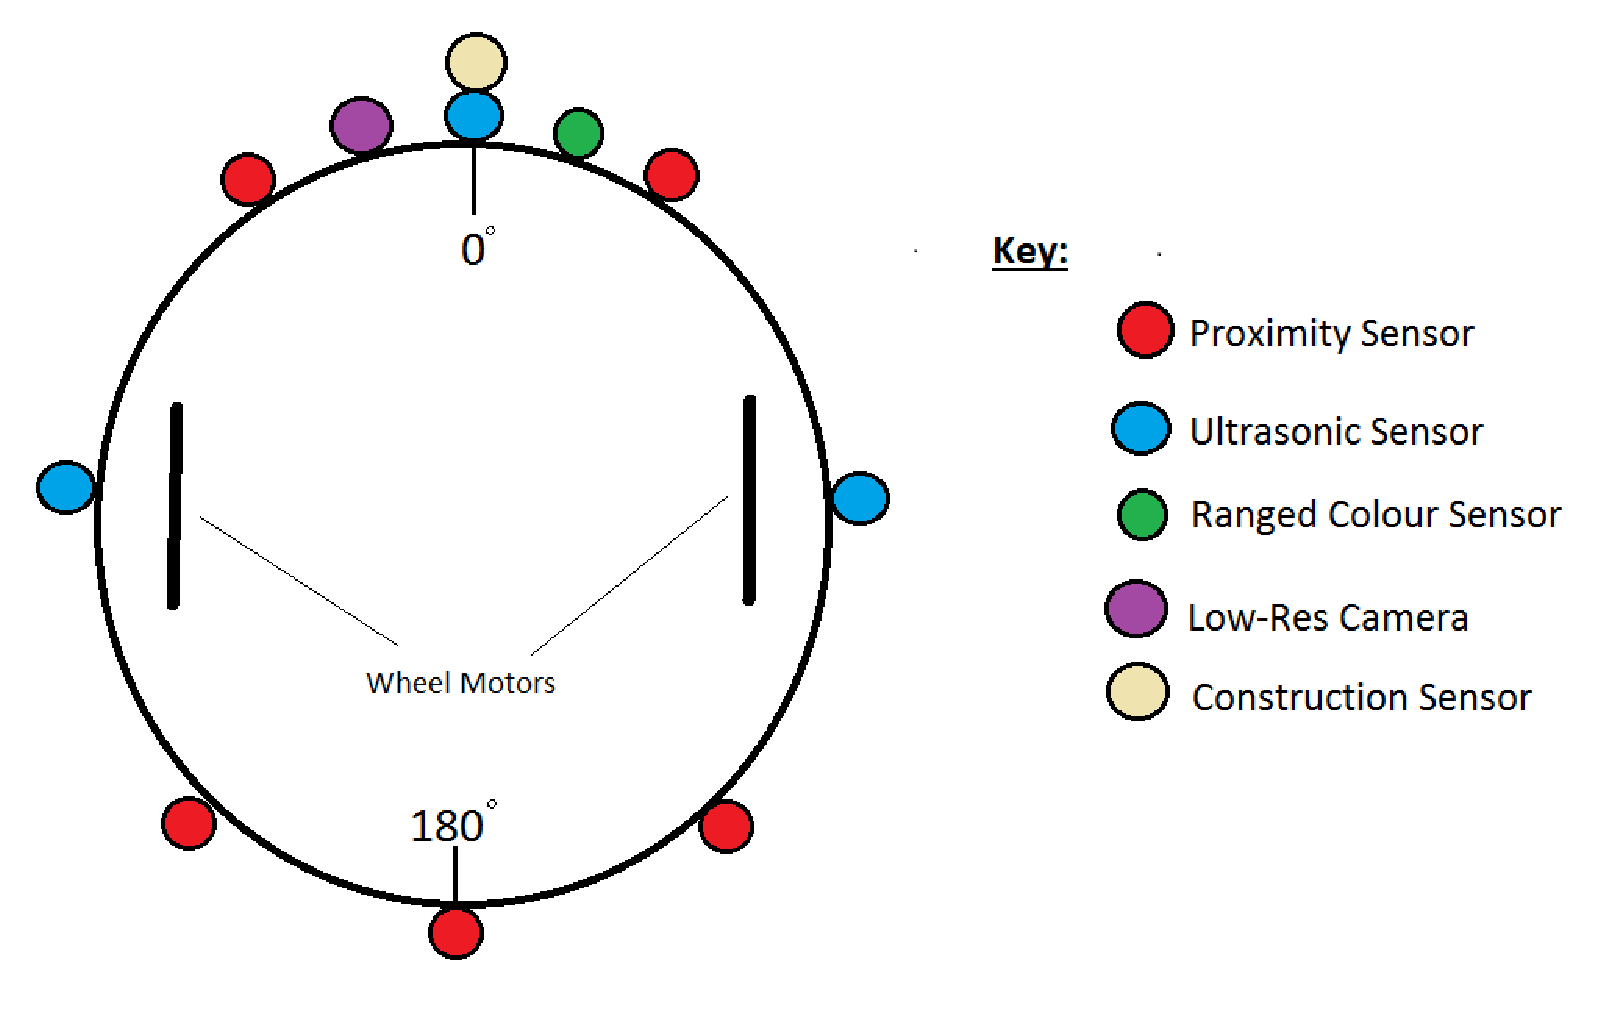
\includegraphics[width=\textwidth]{Morphology.eps}
    \end{minipage}
    \centering
    \begin{minipage}{0.60\textwidth}
       	\centering
        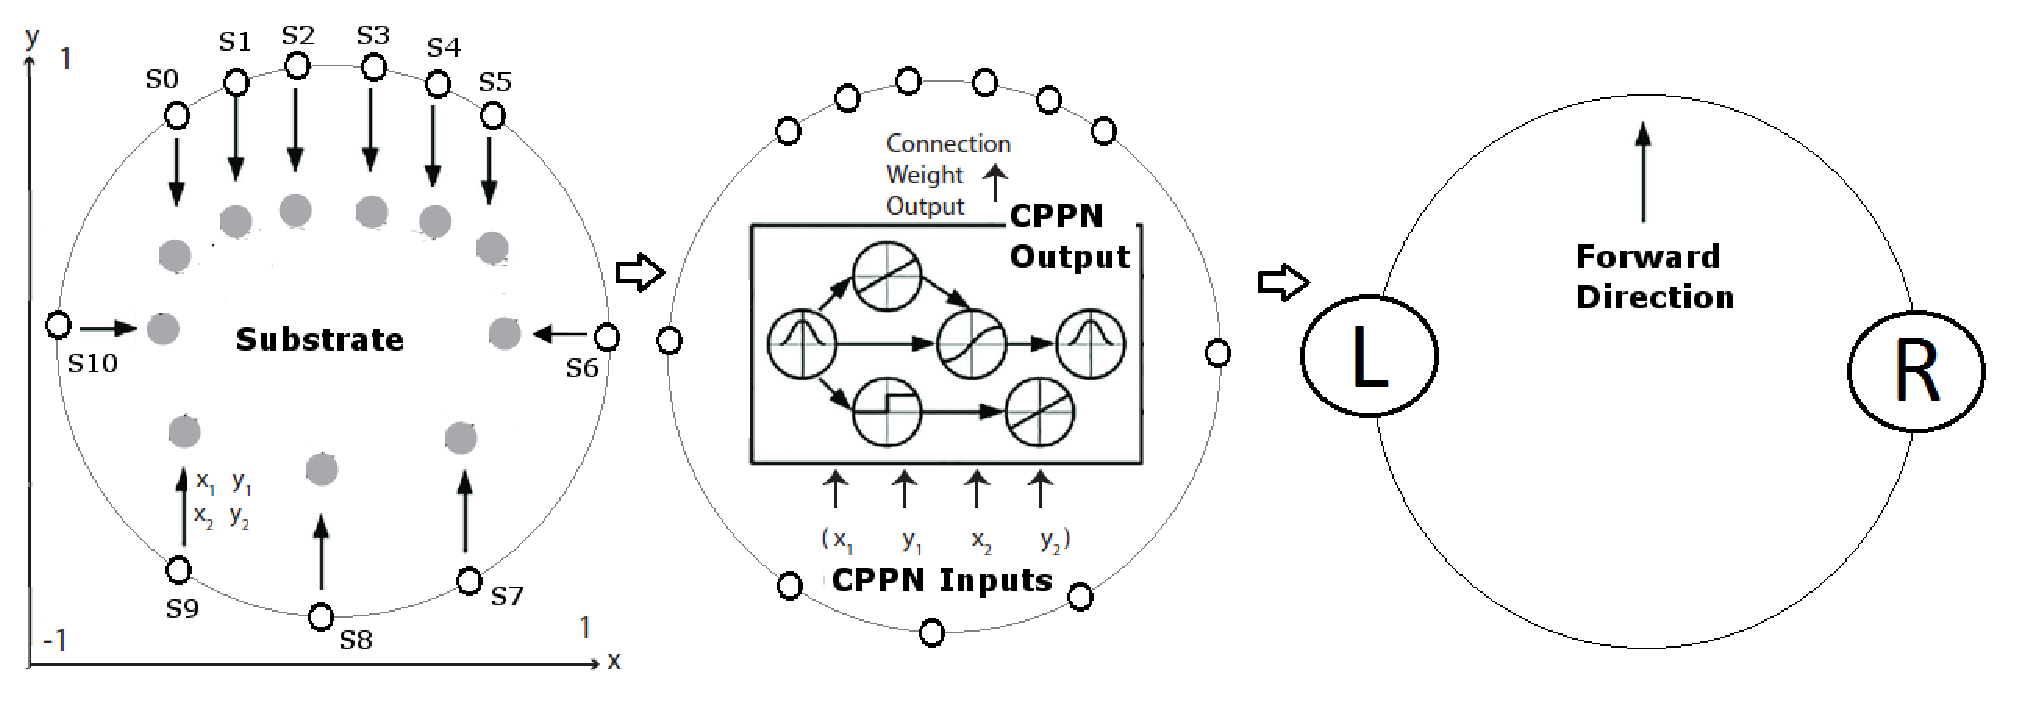
\includegraphics[width=\textwidth]{ANN_Config3.eps}
    \end{minipage}
    \caption{\textit{Left (color):} Robot morphology $1$, with relative positions of various sensors on the robot.
    \textit{Right (gray-scale):} ANN Topology as it relates to robot morphology $1$: $11$ Sensory inputs [S0, S10].  Sensory inputs connect to a hidden
    layer (left).  Connection weight values between two nodes ($x_{1}$, $y_{1}$, $x_{2}$, $y_{2}$) are evolved by querying the CPPN (center) with x, y
    values in the range [-1, 1] (axis shown).  The hidden layer is fully connected to all inputs and outputs (connectivity not depicted).
    Motor outputs (right)
    \textit{L} and \textit{R} determine the speed of the left and right wheels, respectively, and thus a robot's speed and direction.}\label{fig:ann}
\end{figure*}

\section{Methods}

HyperNEAT \cite{StanleyDAmbrosioGauci2009} is an extension of NEAT (\textit{Neuro-Evolution of Augmented Topologies})
\cite{StanleyMiikkulainen2002}, where ANNs are indirectly encoded using a CPPN (\textit{Compositional Pattern Producing Network})
\cite{Stanley2007}.
HyperNEAT was selected as it has a number of benefits demonstrated in previous work \cite{DAmbrosio2013},
\cite{WatsonNitschke2015SSCI}.
This includes its capability to exploit geometric features such as symmetry, regularity and modularity
in robot morphology and the task environment during controller evolution.
%in the  geometric features include the relative positions of other robots, blocks,
%the direction robots and blocks are facing and the shape of the environment.
%Also, the structures to be built are modular
%(comprised of blocks) and often regular (the same sequence of blocks can be repeated).

In this study, HyperNEAT evolves the connection weights between each robot's sensory input layer,
hidden layer and motor output layer, where each robot used the same controller, making teams
homogenous.
Controller evolution experiments were initialized with a given morphology (table \ref{tab:morphConfigs}).
However, in one experiment set, each robot's sensor configuration of team morphology could be
\textit{co-adapted} via HyperNEAT activating and deactivating sensory input node connections over
the evolutionary process.
For these experiments (section \ref{sec:experiments}), \textit{add connection} and
\textit{remove connection} mutation operators (table \ref{tab:simParameters}) from previous work
\cite{HewlandNitschke2015} were applied every generation to a sensory input node
chosen with uniform random selection.  The mutation operator applied depended on whether the chosen input
node was connected or not.  The construction zone sensor (table \ref{tab:morphConfigs}) was permanently activated
for all morphologies and could not be disconnected, as this enabled robots to detect \textit{construction zones}
(section \ref{subsec:constructionTask}).

Table \ref{tab:morphConfigs} presents a list of \textit{morphology identification} (ID) numbers and the
number and type of sensors that correspond to each morphology.
For example, morphology 2 has four proximity sensors, one ultrasonic sensor, one colour-ranged sensor, and
one low-resolution camera.
Note that all morphologies have a construction sensor as this is necessary to complete the collective construction task.

%\vspace{-0.4cm}
\subsection{Robot Team Controller}\label{sec:embodiment}
%\vspace{-0.2cm}
Each robot in the team used an ANN controller with
\textit{N} sensory input nodes, determined by the given morphology being evaluated (table \ref{tab:morphConfigs}).
Each robot's controller mapped sensory inputs, via a fully connected hidden layer, to two motor outputs, the
robot's left and right wheels (figure \ref{fig:ann}). %using HyperNEAT \cite{StanleyDAmbrosioGauci2009}.

Figure \ref{fig:ann} illustrates the sensory configuration for \textit{N} = $11$ (morphology $1$), and the
associated substrate and CPPN used by HyperNEAT.
For each robot morphology (table \ref{tab:morphConfigs}), the sensors corresponding to the input layer
of the controller was a circle \textit{N} nodes distributed about a robot's periphery,
where the exact geometric configuration corresponded to the morphology being evaluated
(figure \ref{fig:ann} illustrates morphology
$1$)\footnote{Illustrations of all robot morphologies tested can be found at: \url{https://github.com/not-my-name/SSCI_Paper_Appendix}}.
The intermediate ANN hidden layer reflects the configuration of the input layer, preserving
the geometry of the sensory input layer, that is, the direction of each sensor's FOV (figure
\ref{fig:ann}).
The ANN was initialized with random weights normalized to the range [-1.0, 1.0], with full connectivity between adjacent layers,
however, partial connectivity was evolvable via the CPPN generating a zero weight.
Collectively all sensors approximated up to a $360$ degree \textit{Field of View} (FOV).

The nodes comprising each robot's ANN controller, connected by the CPPN, were placed in the substrate
illustrated in figure \ref{fig:ann}.
Each node in the substrate was placed at specific ($x$, $y$) locations in the two-dimensional geometric space
of the substrate ($x$, $y$ axes were in the range: [-1, 1]).
Connection weights in the controller were evolved via querying the CPPN for the weight of any connection
between two points ($x_{1}$, $y_{1}$) and ($x_{2}$, $y_{2}$) by inputting ($x_{1}$, $y_{1}$, $x_{2}$, $y_{2}$)
into the CPPN, which subsequently output the associated weight.
During HyperNEAT's evolutionary process, the CPPN was evolved via having nodes and connections added and removed, as well
as connection weight values mutated \cite{StanleyDAmbrosioGauci2009}.

Thus, the CPPN evolved a connectivity pattern across the geometry of the ANN via querying all the potential
connections for their weights.
This connectivity pattern was effectively a function of the task and ANN geometry,
which enabled HyperNEAT to exploit the structure (regularity, repetition and symmetry) of the task and robot morphology.
For example, there was symmetry in the robot morphology in terms of the positioning of sensors about each
robot's periphery (figure \ref{fig:ann}) and there was regularity and repetition in the collective construction
task, in terms of repeating block types comprising modular and regular structures.
In the collective construction task, \textit{modularity} was defined as the composition of modular structures
(buildings in construction zones) from a sequence of connected blocks and \textit{regularity} was defined
as the same sequence of blocks repeated in a building.

Previous work has demonstrated that the indirect encoding of an evolved CPPN facilitates the evolution of
robot controllers with increased task performance enabled by a compact representation
of task and robot geometry \cite{DAmbrosioStanley2008}, \cite{WatsonNitschke2015SSCI}.
Table \ref{tab:simParameters} presents the HyperNEAT parameters used in this study, where \textit{delta}
was angle between the ($x_{1}$, $y_{1}$, $x_{2}$, $y_{2}$) positions of nodes in the substrate.
These parameter values were determined experimentally.   All other HyperNEAT parameters not listed in
table \ref{tab:simParameters}, were set as in previous work \cite{DAmbrosioStanley2008}.
%The ANN uses a three dimensional coordinate system for processing \textit{x}, \textit{y}, \textit{z}
%positions in the CPPN in order to generate weight and bias values and connectivity.
%Previous work  also demonstrated that HyperNEAT exploits the sensory-motor node configuration in ANN controllers,
%Nodes for processing sensory inputs correspond to the direction each sensor faces.

\subsubsection{Detection Sensors}
Each robot was equipped with various sensor types, where the exact sensor complement, including the
relative position and direction on the robot depends upon the given experiment
(section \ref{sec:experiments}) and morphology being evaluated (table \ref{tab:morphConfigs}).
Each robot had \textit{N} sensors corresponding to the \textit{N} inputs comprising the robot's
ANN sensory input layer (figure \ref{fig:ann}), each with a range of \textit{r}
(portion of the environment's length).
A robot's sensory FOV was split into \textit{N} sensor quadrants, where all sensors were constantly active
for the duration of the robot's lifetime.
The \textit{nth} sensor returned a value in the normalized range [0.0, 1.0],
in the corresponding \textit{nth} sensor quadrant.
A value of $0.0$ indicated that no blocks were detected and a value of $1.0$ indicated that an object was detected
at the closest possible distance to the given sensor.
%All detection sensor values are

Table \ref{tab:simParameters} presents the different sensor types used in this study, where the functional properties of each sensor
(range and FOV) were abstractions of corresponding physical sensors typically used on the Khepera III robots \cite{khepera3usermanual2013}.
In table \ref{tab:simParameters}, range values are units defined in relation to the environment size ($20$ x $20$)
and FOV values are in radians.
Each morphology also included a special construction zone detection sensor that activated with a value in the range
[0.0, 1.0] whenever a robot came into
contact with a block that must be connected with other already connected blocks.

The construction zone sensor calculated the squared Euclidean norm, bounded by a minimum observation distance, as an
inversely proportional distance between \textit{this} robot and the closest construction zone, where a value of 1.0 indicated the robot (pushing a block)
was in contact with the construction zone and a value of 0.0 indicated that the robot (pushing a block) was the maximum possible
distance from the closest construction zone.
Robots were unable to detect each other, thus all cooperative interactions were \textit{stigmergic} \cite{BeckersHollandDeneubourg1994}
where robots interacted via pushing blocks into the environment's construction zone.
Furthermore, robots had no \textit{a priori} knowledge of the construction schema,
but rather must discover the construction schema rules by trial and error.
Also, once at least two blocks had been pushed and connected together this formed a construction zone (section \ref{subsec:constructionTask}),
that was then visible to each robot's construction zone sensor.
%Each robot has \textit{N} sensors each with a specified range, field of view and bearing (its position on the robot). The subject of these experimental comparisons is the various combinations of these different types of sensors (referred to as sensor morphologies) that are implemented in the different experiments. These sensor morphologies are predetermined by the experimenter and are outlined later on in this table. Robots are unable to detect each other, thus all cooperative interactions are \textit{stigmergic} \cite{BeckersHollandDeneubourg1994}

\begin{table*} [t]
	\renewcommand{\arraystretch}{1.50}
	\caption{Sensory configuration (number of sensors) for each morphology.}\label{tab:morphConfigs}
	\centering
	\begin{tabular}{| c | c | c | c | c | c |}
		\hline
\textbf{Morphology ID} & \textbf{Proximity Sensors} & \textbf{Ultrasonic Sensors} & \textbf{Color Ranged Sensors} & \textbf{Low-Resolution Camera} & 	 \textbf{Construction Zone Sensors} \\
%                       &   Sensors     &   Sensors          &  Sensors         &   Camera          &   Zone Sensors \\
		\hline
		\textbf{1}               &	5 	 	    & 	3  	             &	1               &	1                &	1   \\
		\textbf{2}               &	4 	 	    &	1		         &	1	            &	1                &	1   \\
		\textbf{3}               &	0 	        &	0				 &	1			    &	1                &	1    \\
		\textbf{4}               &	2 		 	&	0	     		 &	1		        &	1                &	1    \\
		\textbf{5}               &	2  	        & 	2				 &  1               &	1                &	1    \\
		\hline
	\end{tabular}
\end{table*}

\subsubsection{Movement Actuators}

Two wheel motors control a robot's heading at constant speed.
Movement is calculated in terms of real valued vectors (\textit{dx}
and \textit{dy}).  Wheel motors (\textit{L} and \textit{R} in figure \ref{fig:ann})
need to be explicitly activated.
A robot's heading is determined by normalizing and scaling its motor
output values by the maximum distance a robot can traverse in one
iteration (table \ref{tab:simParameters}).  That is:

%\begin{equation}\label{equ:contDisCalc}
$\textit{dx} = d_{max} (o_{1} - 0.5)$

$\textit{dy} = d_{max} (o_{2} - 0.5)$
%\end{equation}

Where, $o_{1}$ and $o_{2}$ are the motor output values, corresponding
to the left and right wheels, respectively, producing an output in the range:
[-1.0, 1.0].
These output values indicate how fast each respective wheel must turn.
Equal output equates to straight forward motion and unequal output results
in the robot rotating about its own axis.
The $d_{max}$ value indicates the maximum distance a robot can move in
one simulation iteration (normalized to 1.0, table \ref{tab:simParameters}).

\section{Experiments}\label{sec:experiments}

Experiments\footnote{Source code for all experiments is online at: \url{https://github.com/not-my-name/ExperimentsRerun}}
tested $15$ robots in a bounded two dimensional continuous environment
($20$ x $20$ units) with randomly distributed type \textit{A}, \textit{B} and
\textit{C} blocks (table \ref{tab:simParameters}).
Robots and blocks were initialized with random orientations and positions throughout the environment.
A construction schema (table \ref{tab:taskComplexity}) dictated the sequence of block
types that must be connected together in order that a specific structure be built \cite{NitschkeSaEC2012}.
Figure \ref{fig:taskEnv} presents an example of the team of $15$ robots working to solve the
collective construction task in the simulation environment containing a distribution of five of each
block type (\textit{A}, \textit{B} and \textit{C}), colored blue, green and red, respectively.
Other colored blocks in the environment indicate those already connected in construction zones
(three illustrated).  The purple, blue and green semi-circles emanating from each robot
represent the FOV of active sensors, where the different colors correspond to different
sensor types (table \ref{tab:simParameters}).

As the purpose this study was to demonstrate the morphological robustness of
HyperNEAT evolved controllers for a collective behavior task of increasing complexity,
the first two versions of the collective construction task required no cooperation and some degree of
cooperation, respectively, though any block could be connected to any other block.
Where as, the most complex version of the task required cooperation and block types
to be connected according to a construction schema (table \ref{tab:taskComplexity}).

\begin{figure}[t]
	\centering
	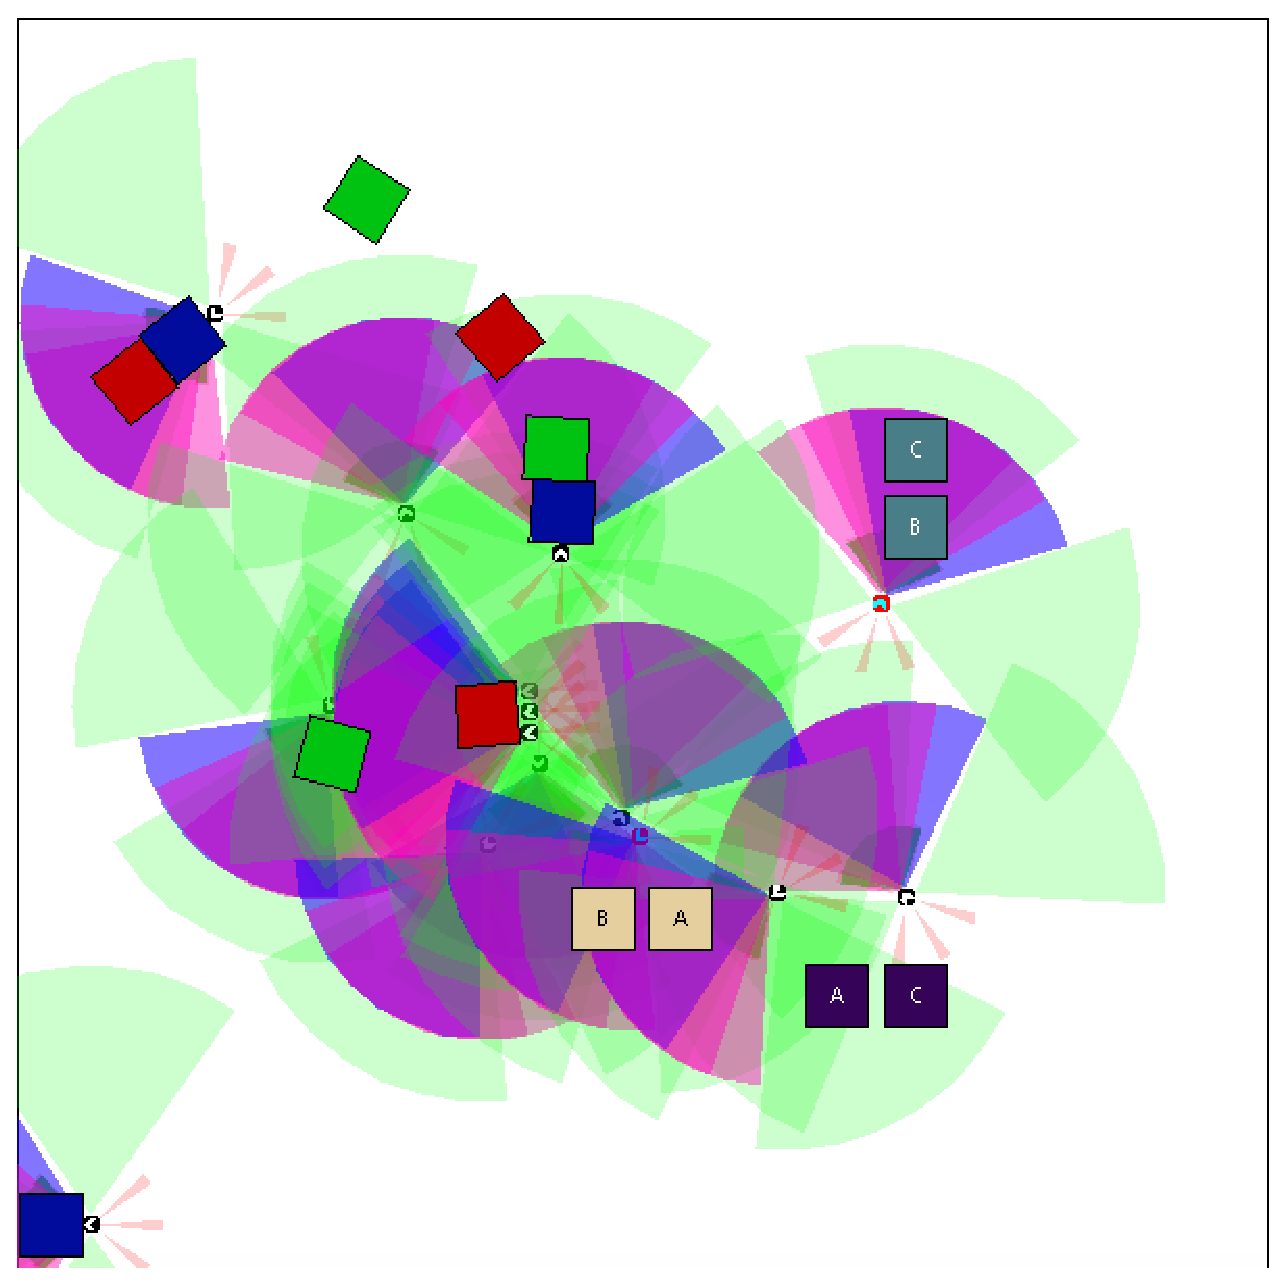
\includegraphics[width=0.40\textwidth]{TaskEnv.eps}
\caption{Example of the simulation environment.  Robots search for randomly distributed
type A, B, and C blocks (blue, green and red, respectively).  Other colored and labeled
blocks indicate those already connected in construction zones.
Different coloured semi-circles emanating from each
robot represent the field of view of currently active different sensor types (table \ref{tab:simParameters}).}\label{fig:taskEnv}
\end{figure}

\begin{figure}[t]
	\centering
	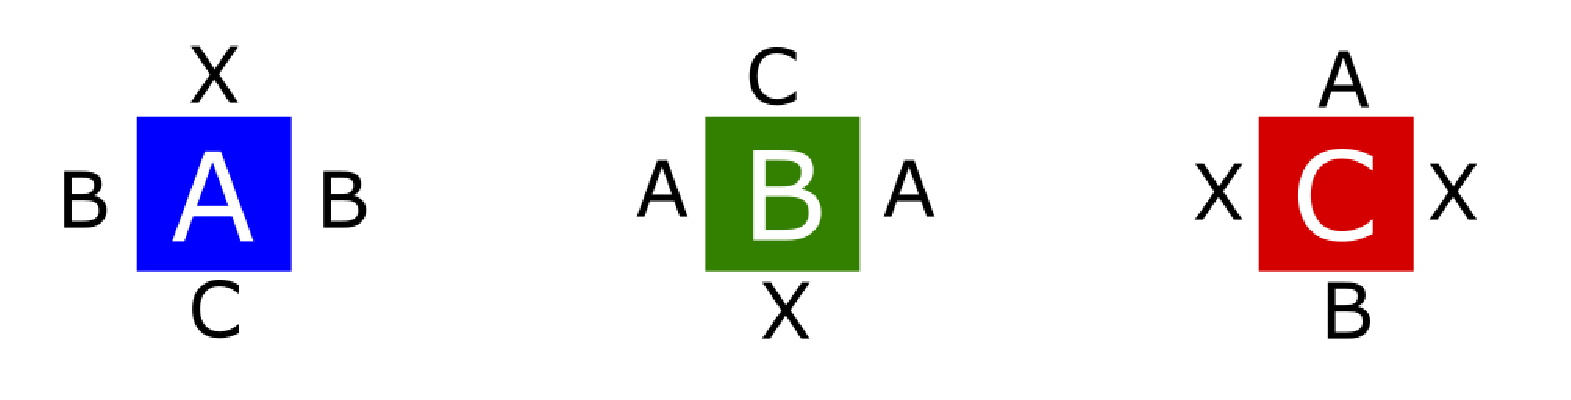
\includegraphics[width=0.5\textwidth]{ConstructionSchema.eps}
	\caption{Task level 3 construction schema: \textit{A}, \textit{B}, and \textit{C} are the block types.  The label on
each side of each block type indicates what block type can be connected to this side.  An \textit{X} label indicates
that no block can be connected.}\label{fig:constructionSchema}
\end{figure}

\subsection{Collective Construction Task}\label{subsec:constructionTask}
This task required the robot team to search the environment for building-blocks and
cooperatively push them together in order that they connected to form a structure,
where connected blocks then formed a construction zone.
Task complexity was equated with the degree of cooperation required to collectively
push blocks and connect them together in the construction zone and whether or not
a construction schema was required.
In this construction task, there were three block types, \textit{A}, \textit{B} and \textit{C}
requiring one, two and three robots to push, respectively.
Cooperation occurred when at least two robots simultaneously pushed a type \textit{B} block,
or at least three robots pushed a type \textit{C} block.

Table \ref{tab:taskComplexity} presents the three levels of task complexity for the
collective construction task.  Level $1$ was the least complex as it did not require
any cooperation, given that it in this case there were only type \textit{A}
blocks in the environment.
Level $2$ was of medium complexity as there are equal numbers of type \textit{A},
\textit{B}, and \textit{C} blocks in the environment, where block types \textit{B} and \textit{C} required
at least two and three robots to push, respectively.
Level $3$ was the most complex, as it required the same degree of cooperation as task level
$2$, though blocks had to be connected according to a construction schema.
Figure \ref{fig:constructionSchema}
illustrates this construction schema, where the label on each of the
four sides of each block type indicates what other block type can be connected to the given side.
The \textit{X} label indicates that no block can be connected to a given side.

The construction zone was formed via at least two blocks pushed together and
was thus any structure being built in the environment.
Once a construction zone was created, all blocks attached to it were fixed in position
and could not be disconnected.
The task mandated a maximum of three construction zones and unconnected blocks
had to be pushed and connected to one of these construction zones.
For task levels $1$ and $2$, any block could be connected to any other block,
meaning that when two blocks were pushed
together they automatically connected.
For task level $3$, blocks had to be pushed together such
that they were connected on specific sides according to the construction schema
(figure \ref{fig:constructionSchema}).

Team task performance was calculated as the number of blocks connected in construction zones
during a team's lifetime (equation \ref{equ:FitnessFunction}),
where average task performance was calculated as the highest task
performance selected at the end of each run ($100$ generations) and averaged over $20$ runs
(table \ref{tab:simParameters}).
The fitness function to direct controller evolution was a weighted sum of
the number of times \textit{type A} blocks were pushed by \textit{one robot}
and connected (\(a\) in equation \ref{equ:FitnessFunction}), the number of times \textit{type B} blocks were pushed
by \textit{two robots} and connected (\(b\) in equation \ref{equ:FitnessFunction}),
and the number of times \textit{type C} blocks were pushed by \textit{three robots}
and connected (\(c\) in equation \ref{equ:FitnessFunction}).

\begin{equation}\label{equ:FitnessFunction}
	f = r_a a + r_b b + r_c c
\end{equation}

Parameter tuning experiments found that setting the weights (reward values \(r_a\), \(r_b\) and \(r_c\))
in equation \ref{equ:FitnessFunction} to 0.3, 0.6, and 1.0, respectively, resulted in functional controller evolution.
Fitness was normalized to the range \([0.0, 1.0]\) using the maximum possible fitness yielded from
all blocks being pushed and connected in construction zones.
%\hlcyan{this is the new content}
%Fitness was normalized to the range \([0.0, 1.0]\) using the total number of each type of block present in the task scenario.

\begin{table}
	\renewcommand{\arraystretch}{1.30}
	\caption{Experiment, Neuro-evolution and Sensor Parameters}\label{tab:simParameters}
	\centering
	\begin{tabular}{llc}
		\hline
		Generations	                                           & 100	\\
		Sensors per robot                                      & 11, 8, 4, 6, random \\	
		Evaluations per genotype                               & 5  \\
		Experiment runs                                        & 20 \\
		Environment length, width                              & 20 \\
        Max Distance (Robot movement per iteration)            & 1.0 \\
        Team size                                              & 15 \\
        Team Lifetime (Simulation iterations)                  & 1000 \\	
        Lifetimes per generation                               & 5 \\
        Type A blocks (1 robot to push)                        & 15 \\
        Type B blocks (2 robots to push)                       & 15 \\
        Type C blocks (3 robots to push)                       & 15 \\
		\hline
		\multirow{4}{*}{Mutation rate} & Add neuron            & 0.25 \\
		& Add connection                                       & 0.008  \\
		& Remove connection                                    & 0.002 \\
		& Weight                                               & 0.1  \\
		Population size                                        & 150 \\
		Survival rate                                          & 0.3 \\
		Crossover proportion                                   & 0.5 \\
		Elitism proportion                                     & 0.1 \\
		CPPN topology                                          & Feed-forward           \\
		CPPN inputs                                            & Position, delta, angle \\
		\hline
		Sensor                                                 & Range     & FOV \\
		\hline
		Proximity Sensor		                               & 	1.0	   &  0.2  \\
		Ultrasonic Sensor		                               &	4.0    &  1.2  \\
		Ranged Colour Sensor	                               &	3.0	   &  1.5 \\
		Low-Res Camera			                               & 	3.0	   &  1.5 \\
		Colour Proximity Sensor                                & 	3.0	   &  3.0 \\
		\hline
	\end{tabular}
\end{table}

\begin{table}[t]
	\renewcommand{\arraystretch}{1.30}
	\caption{Task Complexity. Note: Task level 3 includes a construction schema (figure \ref{fig:constructionSchema}).}\label{tab:taskComplexity}
	\centering
	\begin{tabular}{lccc}
		\hline
		Construction Task Complexity                               & Level 1     & Level 2    & Level 3   \\
		\hline
		Type A blocks (1 robot to push)	                           & 	15	     & 5          & 5  \\
		Type B blocks (2 robots to push)		                   &	0 	     & 5          & 5  \\
		Type C blocks (3 robots to push)	                       &  	0	     & 5          & 5  \\
		Construction schema                                        &   No        & No         &	Yes \\
\hline
	\end{tabular}
\end{table}

\subsection{Experiment Design}\label{subsec:expDesign}

Experiments evaluated the \textit{morphological robustness} of HyperNEAT evolved controllers for
robot teams that must accomplish collective construction tasks of increasing
complexity (section \ref{subsec:constructionTask}).
We measured the average comparative task performance of controllers evolved
for a given team morphology and task complexity where such controllers were
then transferred to
and re-evaluated in other team morphologies.
Thus, teams that achieved an average task performance that was not significantly lower
across all \textit{re-evaluated} morphologies were considered to be \textit{morphologically robust}.

This study comprised five experiment sets, where the first four experiment sets evolved
controllers given team morphologies $1-4$ (table \ref{tab:morphConfigs})
for three levels of increasing task complexity (table \ref{tab:taskComplexity}).
The fifth experiment set investigated the \textit{co-adaptation} of team morphology
and behavior, where morphology $5$ (table \ref{tab:morphConfigs}) was used
as the initial sensory configuration for all robots in the team.
This fifth experiment set was included in order to gauge if co-adapting behavior
and morphology yielded any benefits in this collective construction task as it did in related
collective behavior tasks \cite{HewlandNitschke2015}.

Each experiment set comprised a controller evolution stage and a re-evaluation stage
(morphological robustness test).
For controller evolution, each experiment applied HyperNEAT to evolve team behavior for
$15$ robots for $100$ generations,
where a generation comprised five team \textit{lifetimes} ($1000$ simulation iterations).
Each team lifetime tested different robot starting positions, orientations, and block locations
in the simulation environment.
The fittest controller evolved for each task level (yielding the highest absolute task performance)
was then \textit{re-evaluated} for morphological robustness in all other morphologies.
For example, the fittest controller evolved for morphology $1$ was re-evaluated in morphologies
$2-4$ and the average task performance calculated across all re-evaluation runs.
%($1$ to $7$ in table \ref{tab:morphConfigs}) for the given task.

Each re-evaluation run was \textit{non-evolutionary}, where controllers were not further evolved,
and each re-evaluation run was equivalent to one team lifetime.
Re-evaluation runs were repeated $20$ times for a given morphology, in order to account for random variations in robot and block
starting positions and orientations.
For each fittest controller, re-evaluated in a given morphology, an average task performance was
calculated over these $20$ runs, and then an overall average task performance was computed for
all re-evaluated morphologies.

As per this study's objectives, these morphological re-evaluation
runs tested how robust the fittest evolved controllers (for a given morphology) were to variations
in that morphology.
Thus, re-evaluating the fittest controllers on other morphologies emulated sensor loss due
to damage or new robot morphologies introduced due to changing task constraints.

\begin{figure*}[t]
	\begin{minipage}{0.5\textwidth}
		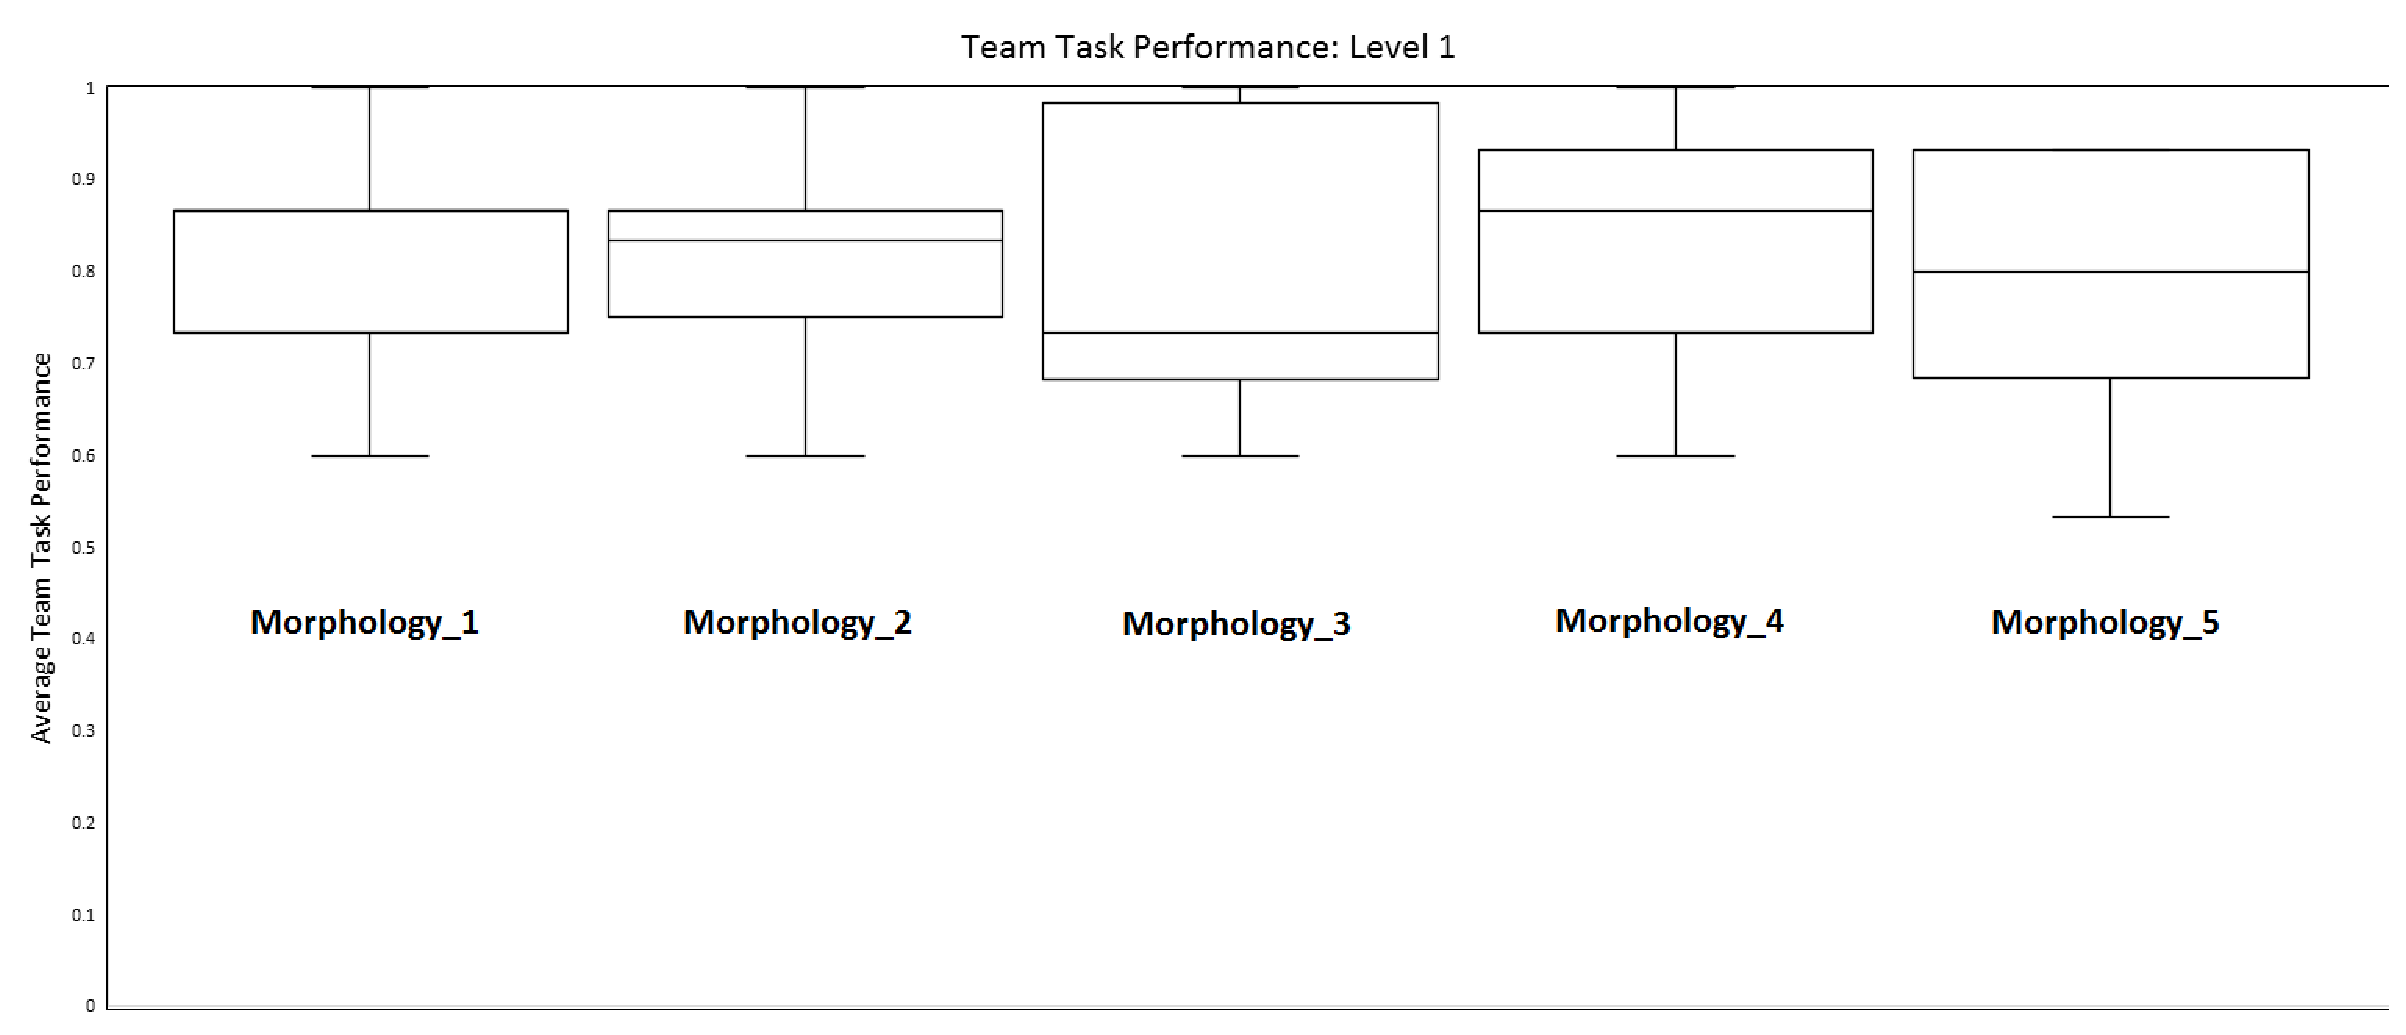
\includegraphics[width=\textwidth]{Evo_BoxPlot_Level1.eps}
	\end{minipage}
	\begin{minipage}{0.5\textwidth}
		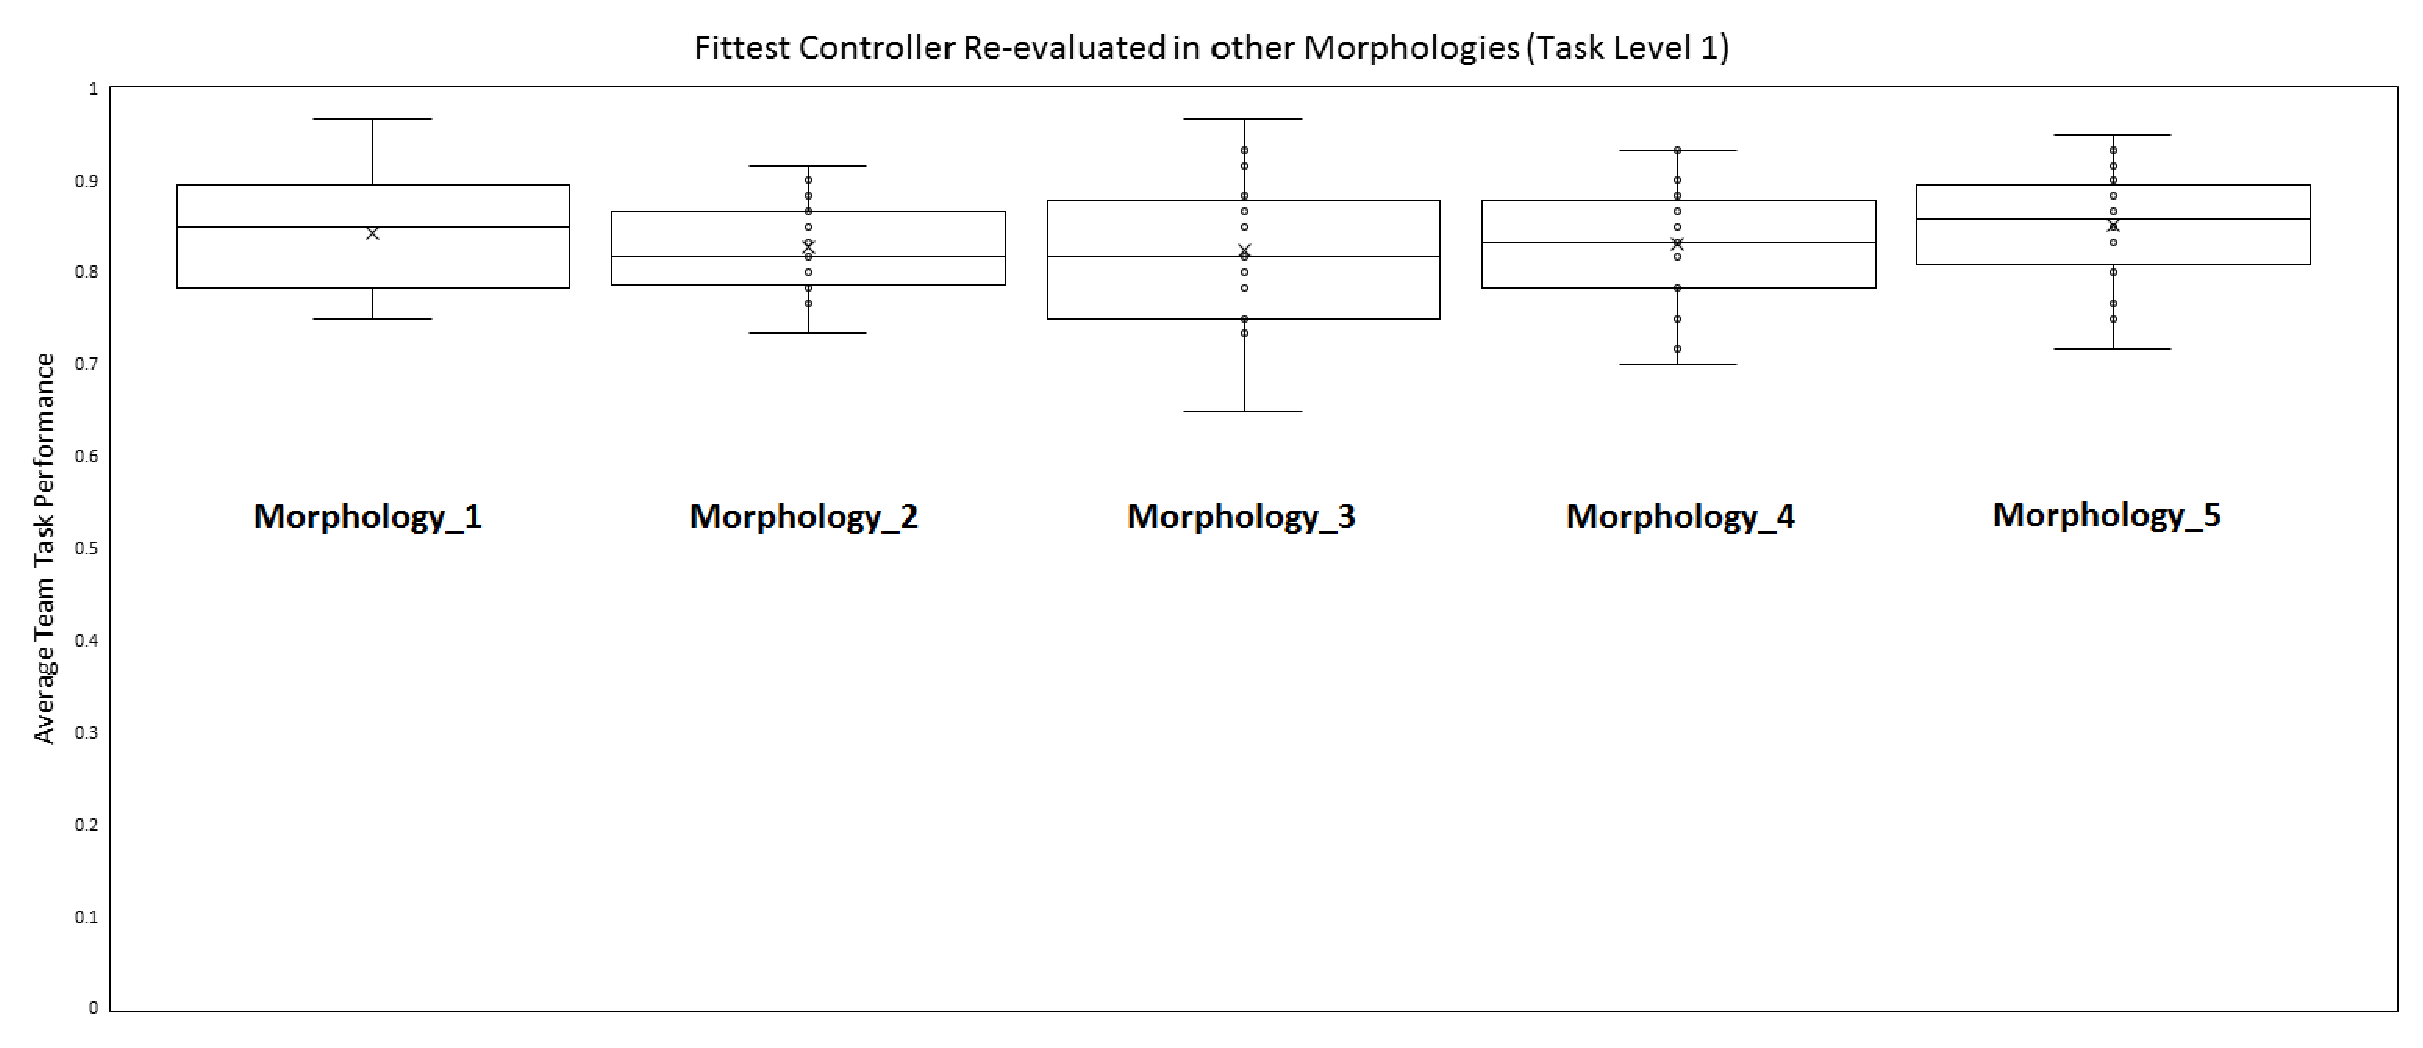
\includegraphics[width=\textwidth]{Level1_ReEval.eps}
	\end{minipage}
\caption{\textit{Left column:} Average team task performance for controller evolution (\textit{task level 1})
given morphologies $1-5$ (depicted from left to right).
\textit{Right column:} Average task performance given the fittest controller evolved
for each successive morphology ($1-5$, shown left to right) re-evaluated in all other morphologies.
For example: Left-most plot is average task performance of fittest controller evolved for
morphology $1$, re-evaluated in morphologies $2-5$.  Right-most plot is the average task performance
of fittest controller evolved for morphology $5$, re-evaluated in morphologies $1-4$.}\label{fig:level1results}
\end{figure*}

\begin{figure*}[t]
	\begin{minipage}{0.5\textwidth}
		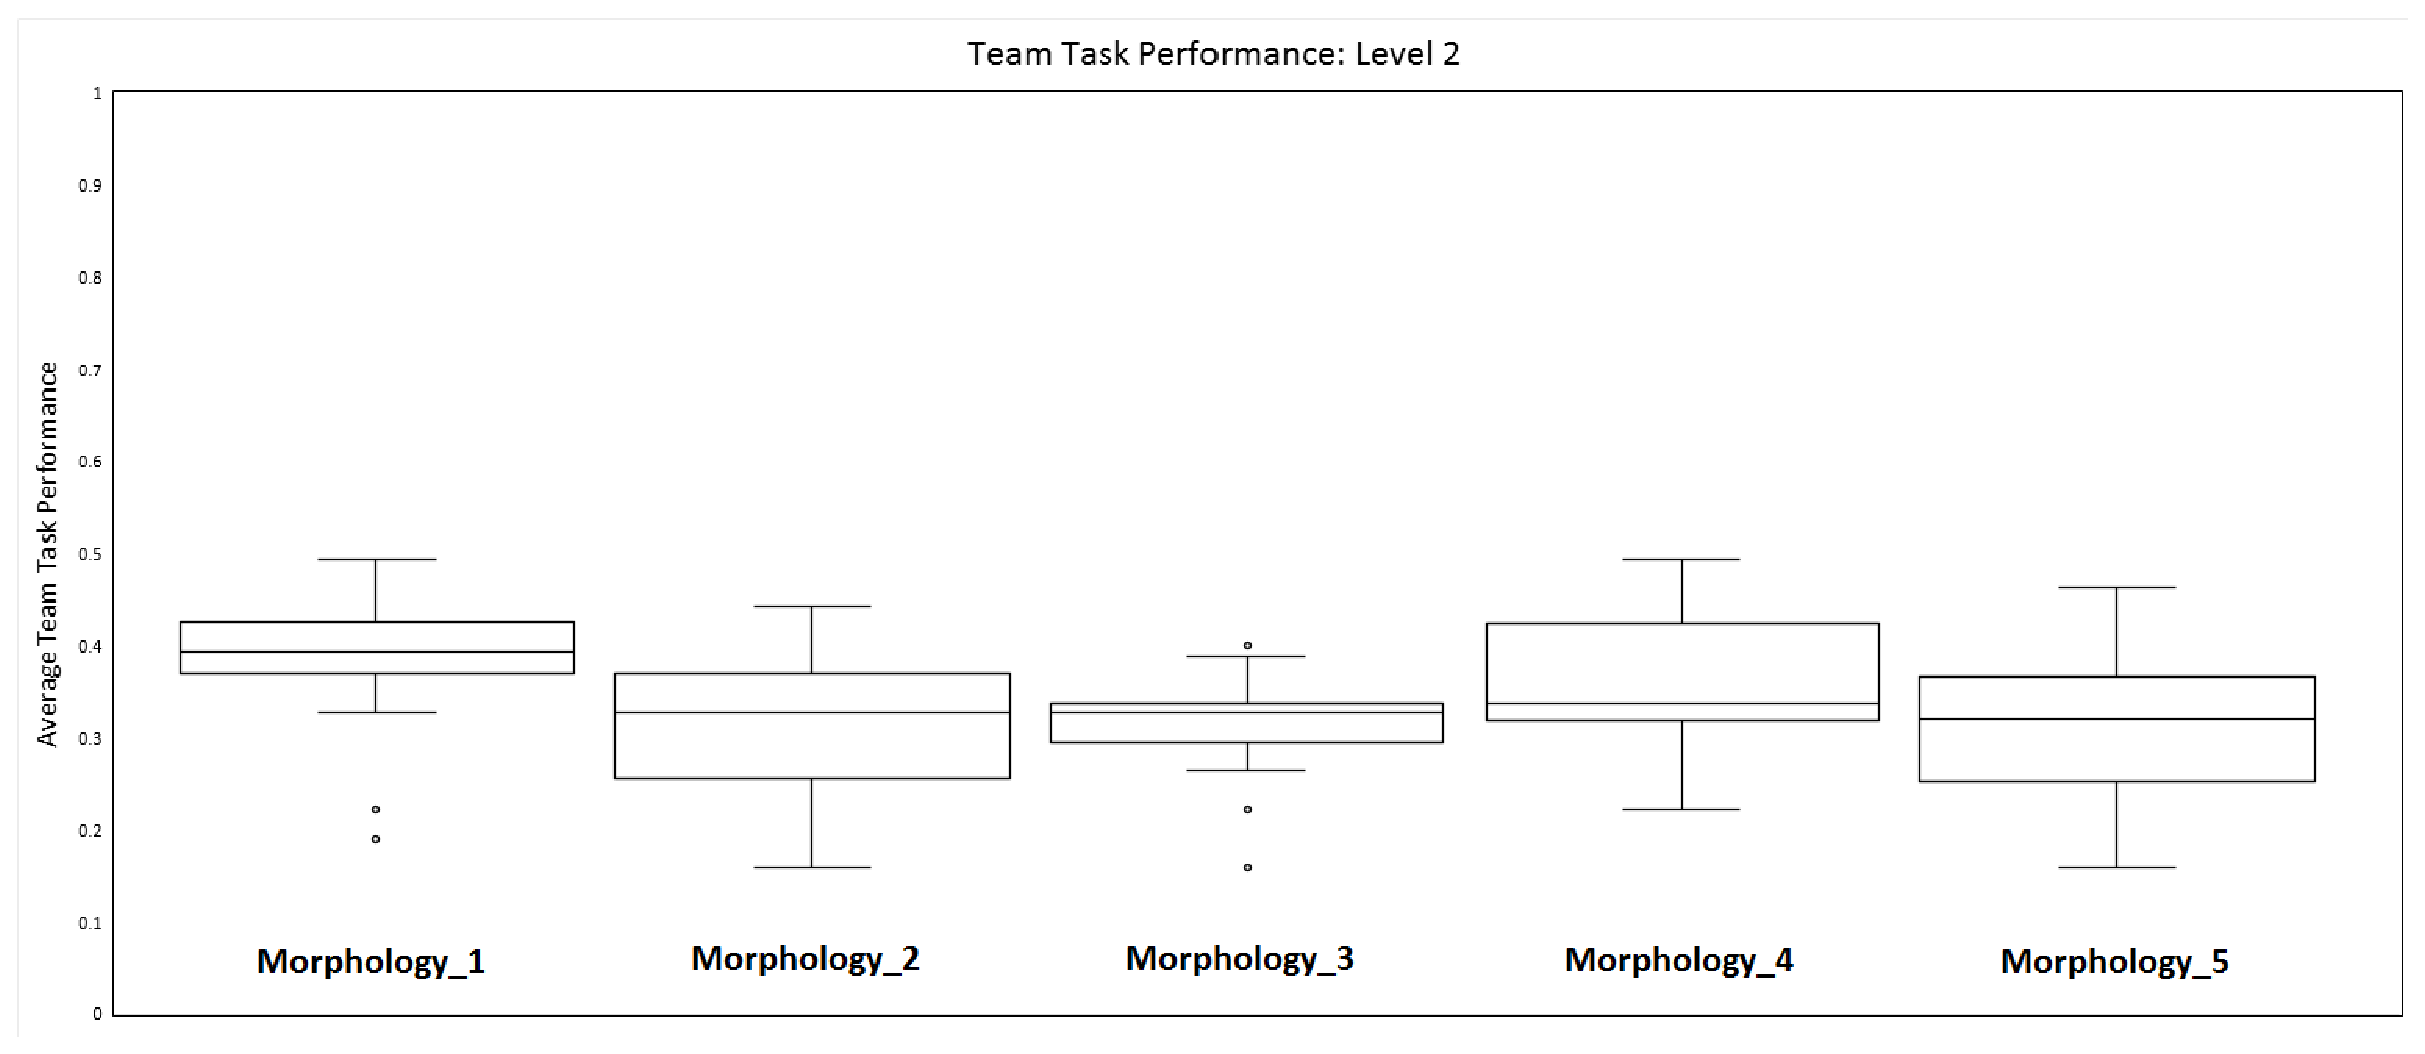
\includegraphics[width=\textwidth]{Evo_BoxPlot_Level2.eps}
	\end{minipage}
	\begin{minipage}{0.5\textwidth}
		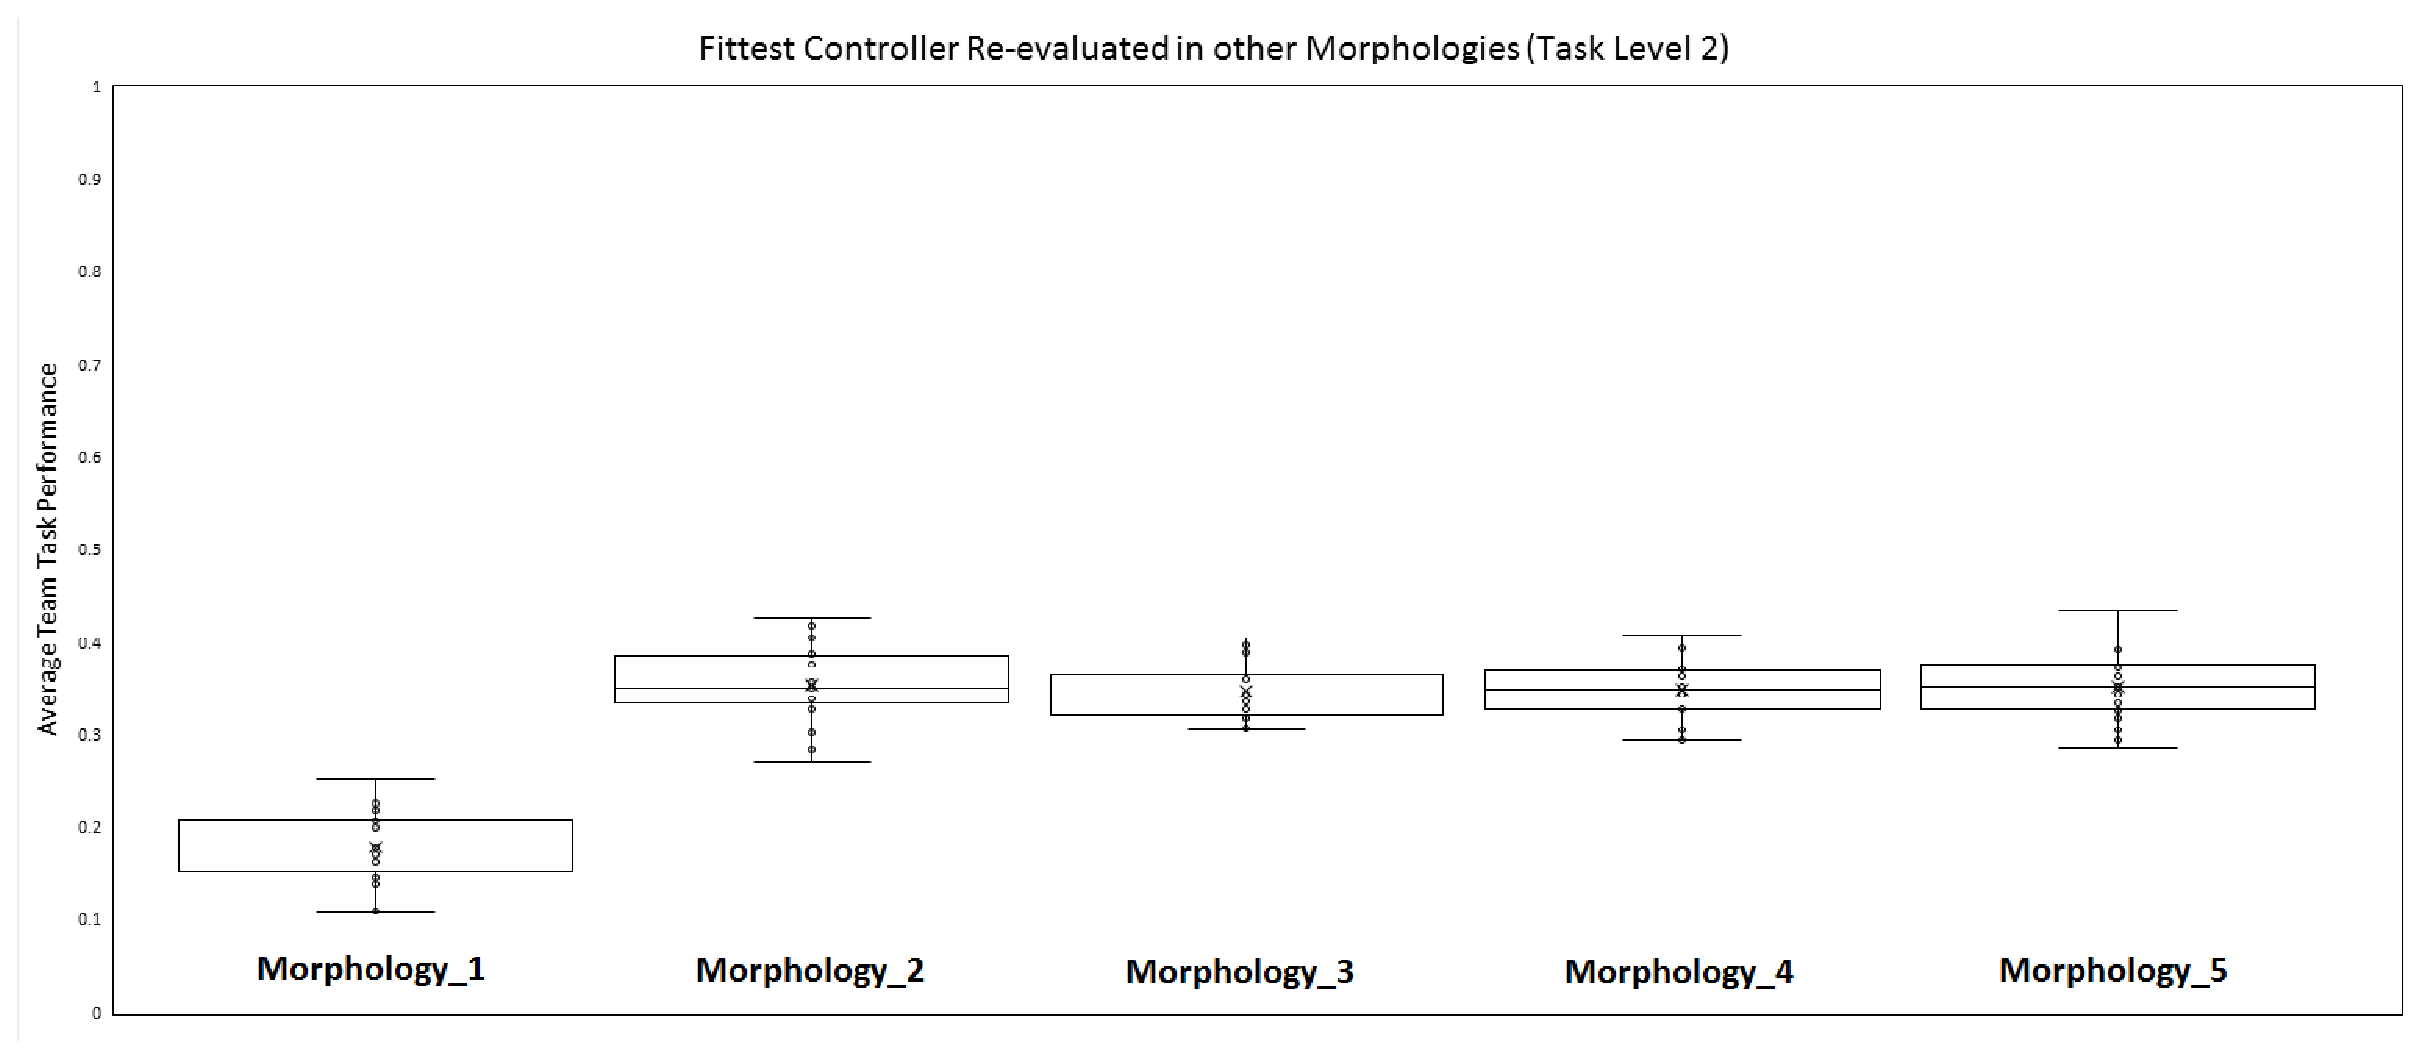
\includegraphics[width=\textwidth]{Level2_ReEval.eps}
	\end{minipage}
\caption{\textit{Left column:} Average team task performance for controller evolution (\textit{task level 1})
given morphologies $1-5$ (depicted from left to right).
\textit{Right column:} Average task performance given the fittest controller evolved
for each successive morphology ($1-5$, shown left to right) re-evaluated in all other morphologies.
For example: Left-most plot is average task performance of fittest controller evolved for
morphology $1$, re-evaluated in morphologies $2-5$.  Right-most plot is the average task performance
of fittest controller evolved for morphology $5$, re-evaluated in morphologies $1-4$.}\label{fig:level2results}
\end{figure*}

\begin{figure*}[t]
	\begin{minipage}{0.5\textwidth}
		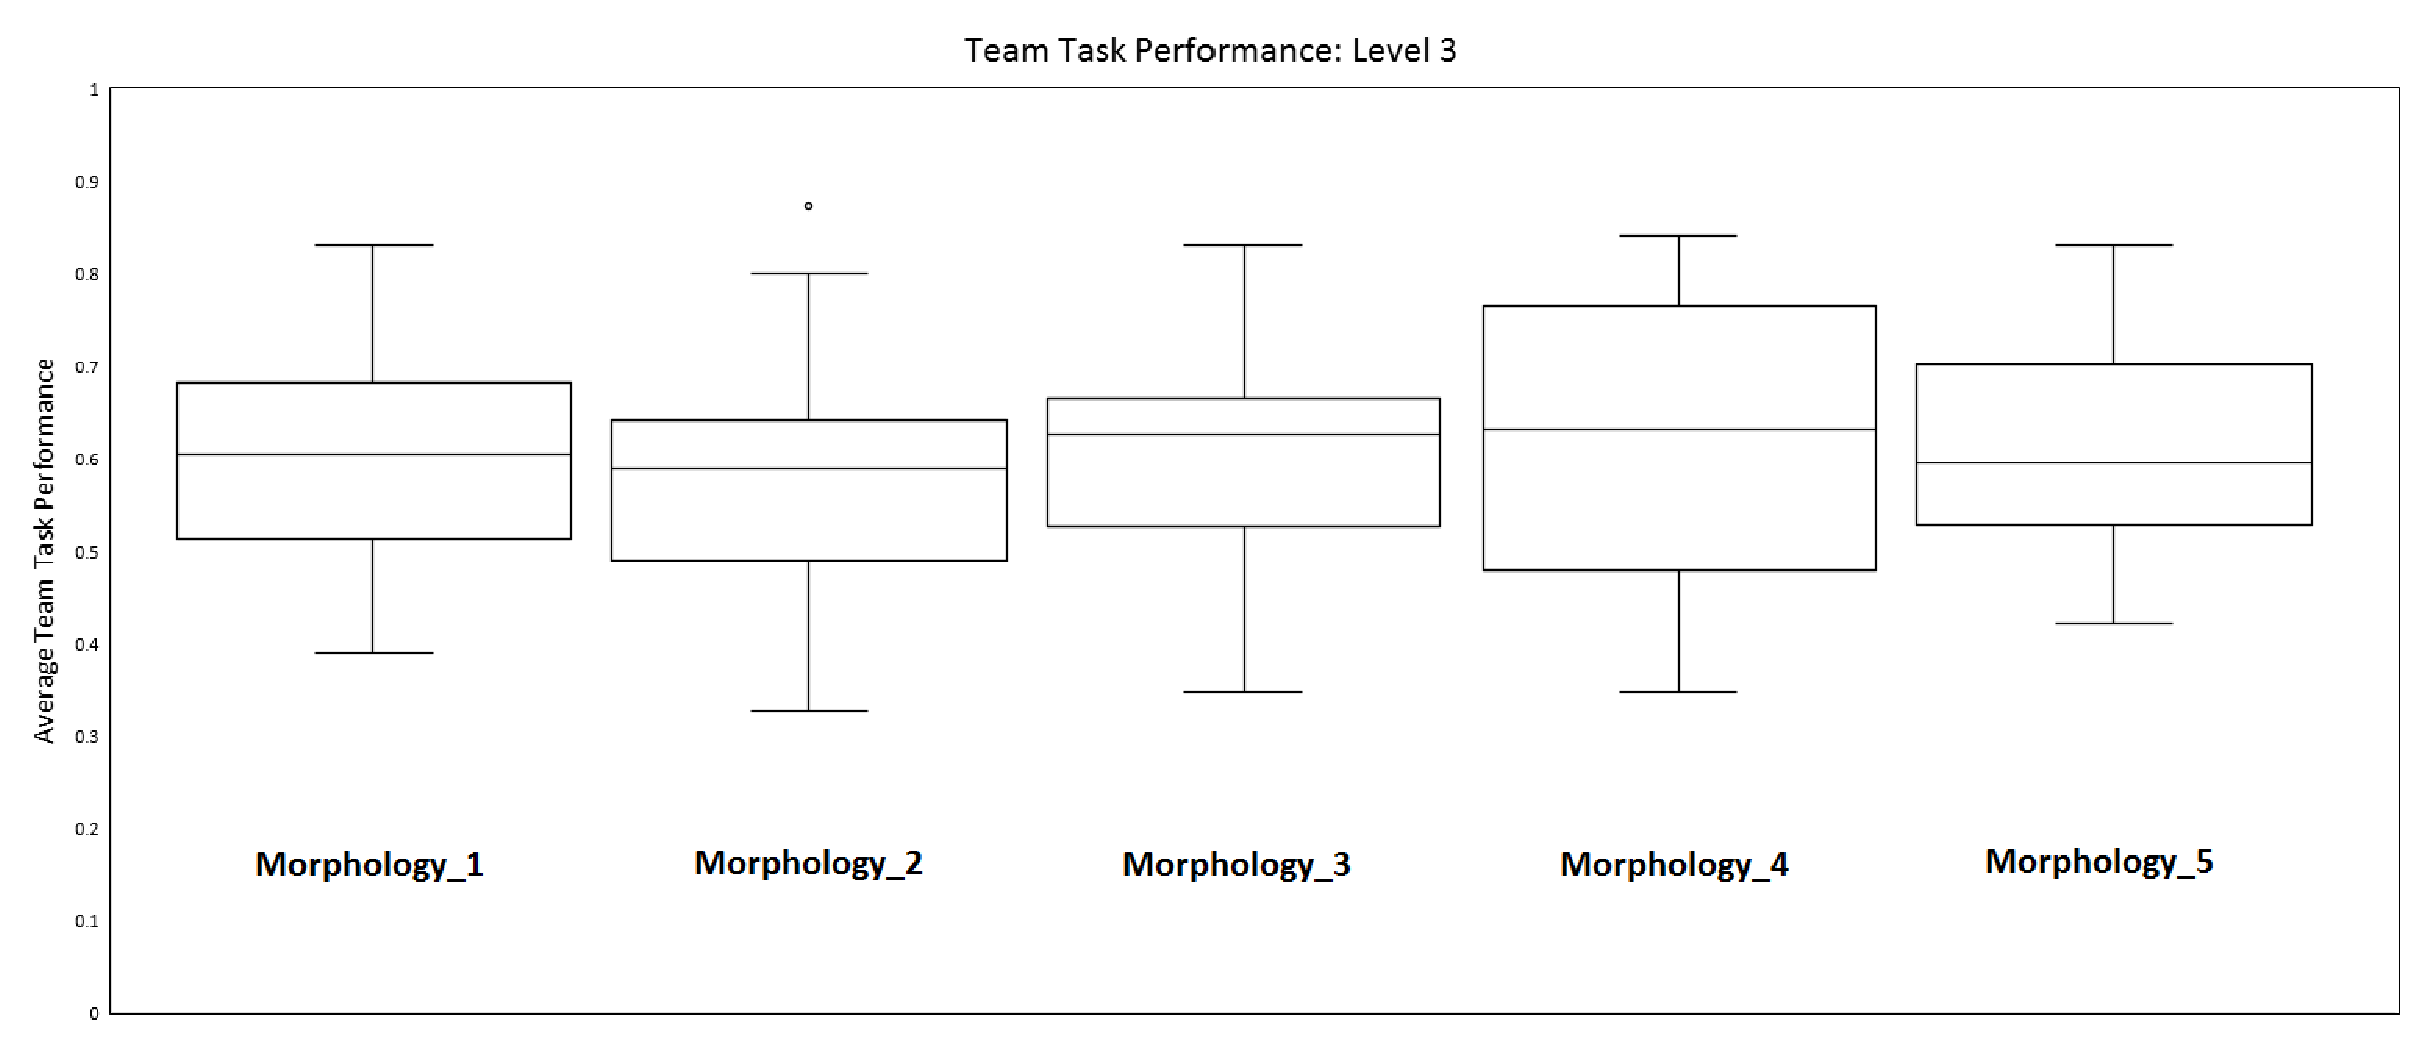
\includegraphics[width=\textwidth]{Evo_BoxPlot_Level3.eps}
	\end{minipage}
	\begin{minipage}{0.5\textwidth}
		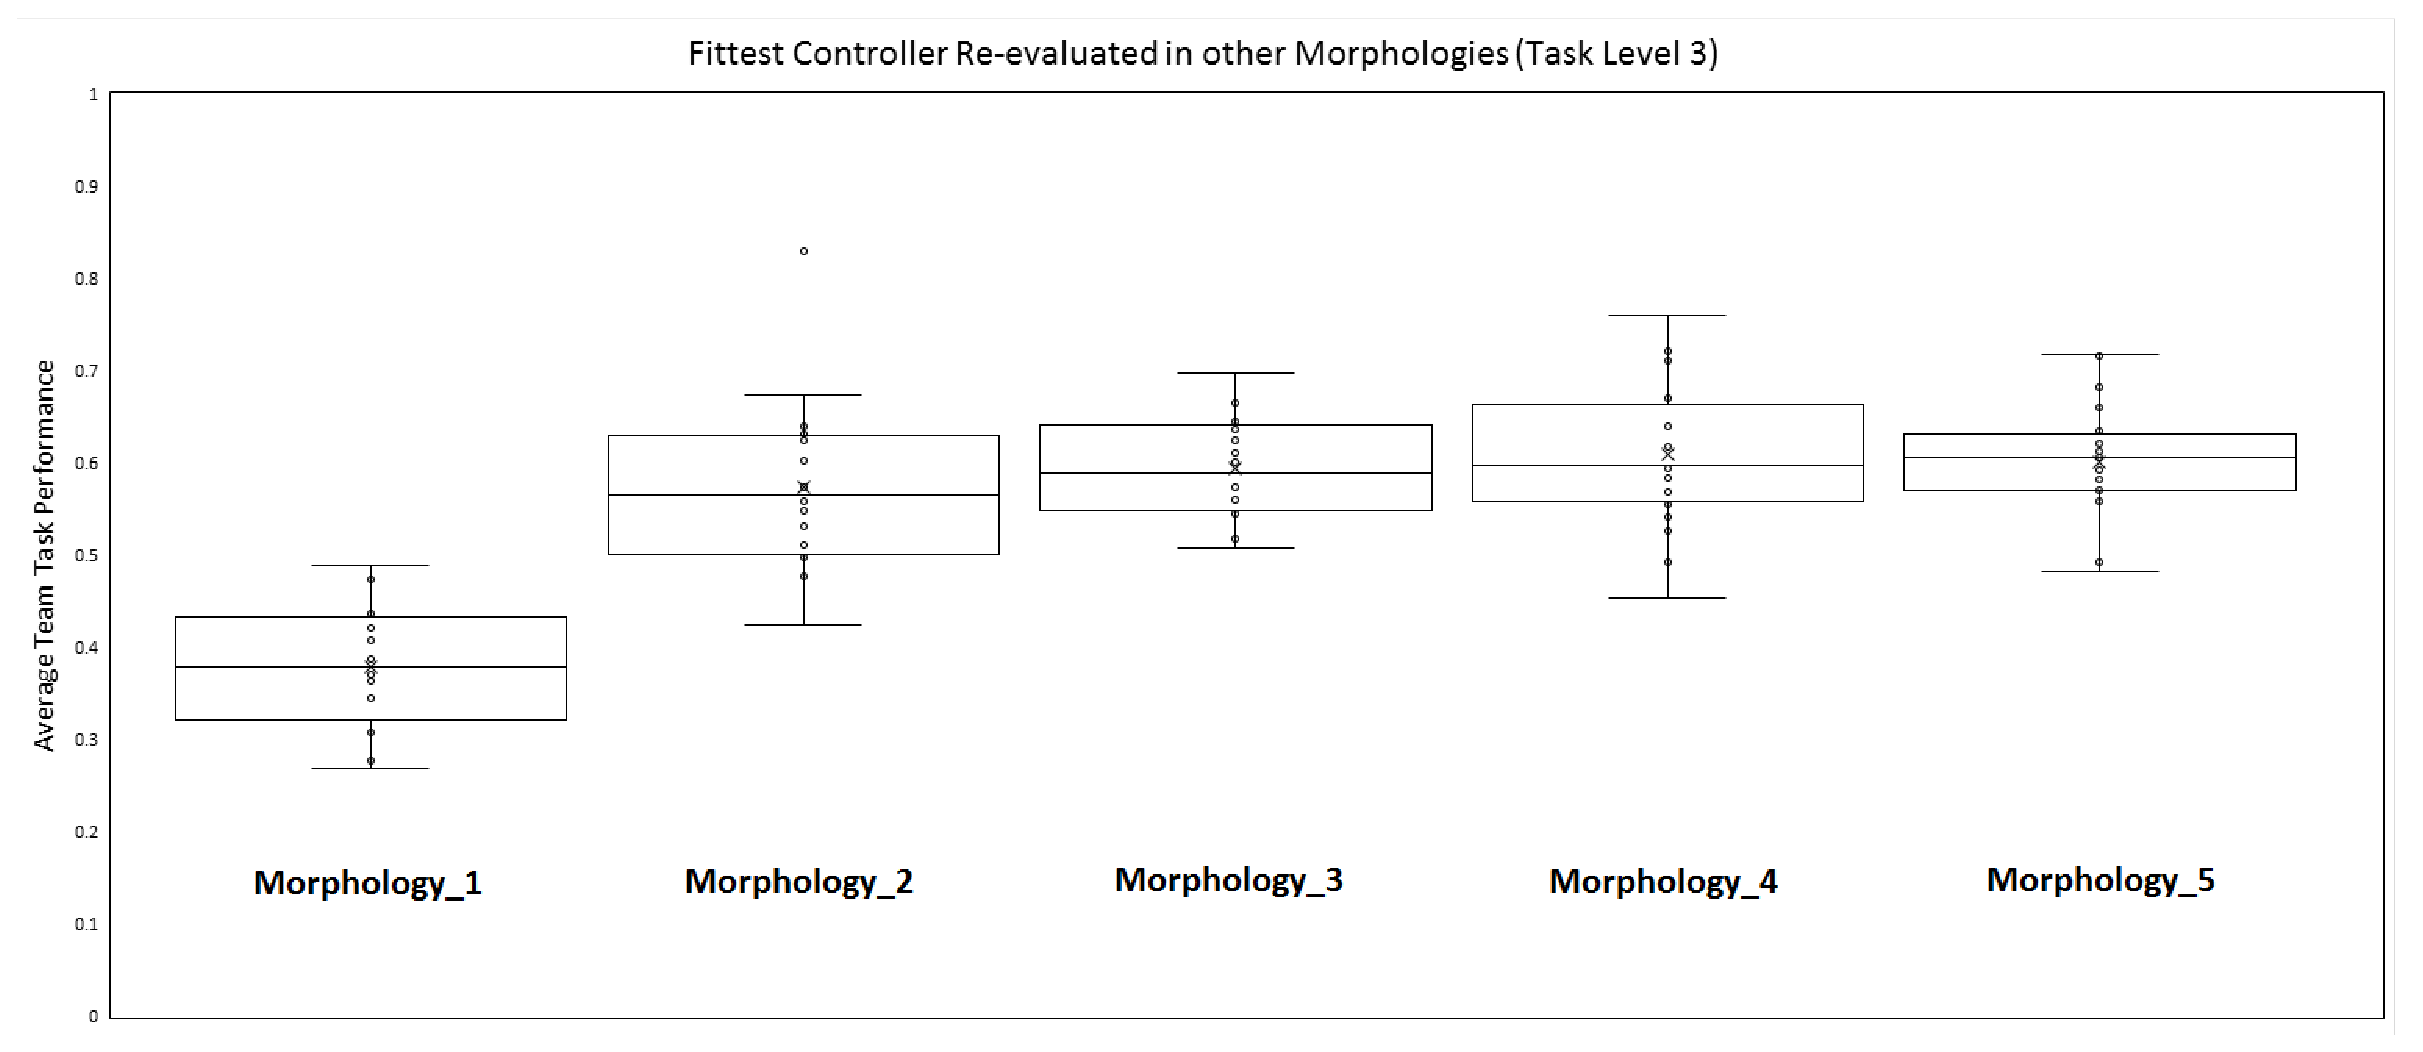
\includegraphics[width=\textwidth]{Level3_ReEval.eps}
	\end{minipage}
\caption{\textit{Left column:} Average team task performance for controller evolution (\textit{task level 1})
given morphologies $1-5$ (depicted from left to right).
\textit{Right column:} Average task performance given the fittest controller evolved
for each successive morphology ($1-5$, shown left to right) re-evaluated in all other morphologies.
For example: Left-most plot is average task performance of fittest controller evolved for
morphology $1$, re-evaluated in morphologies $2-5$.  Right-most plot is the average task performance
of fittest controller evolved for morphology $5$, re-evaluated in morphologies $1-4$.}\label{fig:level3results}
\end{figure*}

%\begin{table}[t]
%	\renewcommand{\arraystretch}{1.30}
%	\caption{Two-way ANOVA: Impact of sensor configuration and task complexity on team performance - Task level 1.}\label{tab:anovaL1}
%	\centering
%	\begin{tabular}{lrrrrr}
%				     &     Df  & SS & MS & F & p \\
%    	\hline
%        Complexity    			&   2  & 27.88  & 13.94 &   1187.36 & \(1.6 \times 10^{-181}\)\\
%        Morphology   	 		&   7  & 3.68   & 0.53 &   44.8 & \(3.9 \times 10^{-48}\)		\\
%        Complexity:Morphology 	&   14 & 2.28   & 0.16 &   13.86 &  \(1.29 \times 10^{-27}\)	\\
%        Residuals     			&   456& 39.19  & 0.12 &          &               \\
%        \hline
%	\end{tabular}
%\end{table}

%\begin{table}[t]
%	\renewcommand{\arraystretch}{1.30}
%	\caption{Two-way ANOVA: Impact of sensor configuration and task complexity on team performance - Task level 2.}\label{tab:anovaL2}
%	\centering
%	\begin{tabular}{lrrrrr}
%								& Df  & SS & MS & F & p \\
%		\hline
%		Complexity    			&   2 & 17.81 & 8.92 &   649.21 & \(3.8 \times 10^{-134}\)\\
%		Morphology   	 		&   7 & 0.19 & 0.03 &   1.98 &  0.06		\\
%		Complexity:Morphology 	&   14 & 0.15 & 0.01 &   0.79 &  0.68	\\
%		Residuals     			& 456 & 6.26 & 0.01 &          &               \\
%		\hline
%	\end{tabular}
%\end{table}

%\begin{table}[t]
%	\renewcommand{\arraystretch}{1.30}
%	\caption{Two-way ANOVA: Impact of sensor configuration and task complexity on team performance - Task level 3.}\label{tab:anovaL3}
%	\centering
%	\begin{tabular}{lrrrrr}
%								& Df  & SS & MS & F & p \\
%		\hline
%		Complexity    			&   2 & 24.67 & 12.34 &   920.91 & \(7.3 \times 10^{-161}\)\\
%		Morphology   	 		&   7 & 0.25 & 0.04 &   2.69 &  0.01 \\
%		Complexity:Morphology 	&   14 & 1.49 & 0.11 &   7.94 &  \(3.41 \times 10^{-15}\)	\\
%		Residuals     			& 456 & 6.11 & 0.01 &          &         \\
%		\hline
%	\end{tabular}
%\end{table}

\section{Results \& Discussion}

For each controller evolution experiment, the average maximum task performance
of controllers evolved for a given morphology and level of task complexity, was recorded.
Specifically, this task performance was calculated by running the absolute fittest controller
evolved after $20$ evolutionary runs (for a given a morphology and task level),
in the same morphology over $20$ non-evolutionary runs.
This is presented in figures \ref{fig:level1results}, \ref{fig:level2results} and \ref{fig:level3results}
(left column), where controllers were evolved given morphologies $1$-$5$ (table \ref{tab:morphConfigs}).
In figures \ref{fig:level1results}, \ref{fig:level2results} and \ref{fig:level3results} (left column),
these results are presented from left to right.
For example, average task performance results for morphology $1$ are plotted on the left-most side
and average task performance results for morphology $5$ are plotted on the right-most side.

For each re-evaluation experiment, the fittest controller evolved for a given morphology and task complexity
level was re-evaluated in all other morphologies (for the same level of task complexity), and an
average task performance computed over $20$ runs.
These morphological re-evaluation results are presented in figures \ref{fig:level1results}, \ref{fig:level2results}
and \ref{fig:level3results} (right column).
Each of the five plots (from left to right) in each figure corresponds to the fittest controller evolved for each of the
five morphologies and re-evaluated in all other morphologies.  For example, the left-most plot presents
the average task performance of the fittest controller evolved in morphology $1$ and re-evaluated on morphologies $2-5$.
Where as, the right-most plot presents the average task performance of the fittest controller evolved given morphology $5$
(as the initial sensory configuration) and re-evaluated on morphologies $1-4$.

To gauge the impact of a given team morphology (table \ref{tab:morphConfigs})
in company with a given level of task complexity (table \ref{tab:taskComplexity}),
the \textit{t-test} \cite{FlanneryTeukolsky1986} ($p < 0.05$),
was applied in pair-wise comparisons between sets of controller evolution
results\footnote{Statistical test results for pair-wise comparisons for the fittest evolved controllers
(for a given morphology) tested in each other morphology (individually) is online at:
\url{https://github.com/not-my-name/SSCI_Paper_Appendix}}
(figures \ref{fig:level1results}, \ref{fig:level2results} and \ref{fig:level3results}, left column).
Within each given level of task complexity, no statistically significant difference was found between
controllers evolved given morphologies $1-5$ (controller evolution experiments $1-5$).
Controller evolution experiments $1-4$ were those implementing controller evolution in fixed sensory
configurations (morphologies $1-4$).  Where as, controller evolution experiment $5$ used morphology $5$
as the initial sensory configuration and subsequently co-adapted behavior (controller) and morphology
(complement of sensors).
The lack of statistical difference between controllers evolved given morphologies $1-4$ (table \ref{tab:morphConfigs})
indicates that these sensory configurations were not sufficiently different so as to result in
significantly different average maximum task performances.
Also, the lack of any significant difference between the average maximum task performance of controllers
evolved given morphologies $1-4$ and behavior-morphology co-adaptation (starting with morphology $5$),
supports previous results demonstrating that behavior-morphology co-adaptation
yields at least comparable task performance benefits (compared to fixed morphology controller evolution)
in collective behavior tasks \cite{HewlandNitschke2015}.

However, to address this study's main objective it was necessary to ascertain the morphological robustness
of the fittest controller evolved in each morphology when re-evaluated in all other morphologies.
To gauge the morphological robustness of the fittest controllers evolved for a given morphology ($1-5$),
and a given task complexity, we applied the t-test in pair-wise comparisons of two result
data sets.  First, the average maximum task performances yielded by controller evolution in morphologies
$1-5$ and second, the average maximum task performances yielded from re-evaluating the fittest controller
evolved for a given morphology in all other morphologies (section \ref{subsec:expDesign}).
%Thus, we also used two-way ANOVA tests to measure the impact of task complexity and re-evaluating the fittest
%controller evolved for each morphology on all morphologies (in comparison to controller evolution results).

Statistical test results indicated no significant difference (with one exception) between average task performance results
yielded by controller evolution and morphological re-evaluation experiments for all task complexity levels.
Specifically, the average maximum task performance yielded by controllers evolved given morphologies $2$-$5$
(figures \ref{fig:level1results}, \ref{fig:level2results}, \ref{fig:level3results}, left column) was not
significantly lower than the average task performance yielded by the fittest controllers
(evolved in morphologies $1-5$), and then re-evaluated on other morphologies
(figures \ref{fig:level1results}, \ref{fig:level2results}, \ref{fig:level3results},
right column).  The exception was morphology $1$ in task complexity levels $2$ and $3$.
In these tasks, the fittest controller evolved for morphology $1$, yielded a significantly higher average
task performance than that yielded when this fittest controller was re-evaluated in
morphologies $2-5$.
%Statistical test results are summarized in tables \ref{tab:anovaL1}, \ref{tab:anovaL2}
%and \ref{tab:anovaL3} for task complexity levels $1$, $2$ and $3$, respectively,
%and include performance results comparisons between controller evolution and
%morphological re-evaluation experiments with respect to task complexity and morphology.

Hence, these results indicate that controllers evolved by HyperNEAT for a given morphology
(table \ref{tab:morphConfigs}), overall have the capacity to continue to effectively operate
when transferred to other morphologies.
This result was found to hold for all four of the five morphologies that controllers were evolved for,
and for all levels of task complexity tested (table \ref{tab:taskComplexity}).
%thus demonstrating the morphological robustness of HyperNEAT evolved controllers.

The efficacy of HyperNEAT for evolving morphologically robust controllers is further supported
by the controller evolution experiments that used morphology $5$ (section \ref{sec:experiments}).
In this case, the number of sensors was adapted meaning that team behavior and
morphology were co-adapted.
Specifically, these controller evolution experiments began with the sensory configuration of
morphology $5$ (table \ref{tab:morphConfigs}) and enabled and disabled sensor connections to
better couple morphology with the evolved controller.  Hence, the fittest
controller evolved in this case often corresponded to a sensory configuration
dissimilar to morphology $5$ (the initial sensory configuration).
Results indicated that the fittest controller evolved for morphology $5$, when re-evaluated in
other morphologies, yielded an average task performance that was statistically comparable to
the average task performance yielded by controller evolution given morphology $5$.
This result was observed for all three task complexity levels
(figures \ref{fig:level1results}, \ref{fig:level2results}, and \ref{fig:level3results}, right column).

Thus, controllers evolved for fixed morphologies ($1-4$, table \ref{tab:morphConfigs}), were
found to be \textit{morphologically robust}, as there was no significant difference in average maximum
task performance when the fittest controller (evolved for morphology $1-4$), was re-evaluated in other
morphologies.
Furthermore, the fittest controller evolved for an adaptive morphology ($5$, table \ref{tab:morphConfigs}),
was similarly found to be morphologically robust, given that the average maximum task performance
yielded when this fittest controller was re-evaluated in other morphologies ($1-4$), was comparable to
the average maximum task performance yielded from morphology $5$ controller evolution experiment.
This is theorized to be a result of the complexity of co-adapting effective controller-morphology
couplings \cite{PfeiferBongard2006} within limited periods of artificial evolution ($100$ generations in these experiments,
table \ref{tab:simParameters}), offset by the transference of evolved
\textit{connectivity patterns} \cite{GauciStanley2010} as functional controllers across varying
robot morphologies  \cite{RisiStanley2013}.
Such connectivity patterns encode behaviors that do not rely upon specific sensory-motor mappings in
controllers and thus do not necessitate specific task environment configurations,
such as specific numbers of agents or objects.
This in turn facilitates the transfer of controllers across varying team morphologies
\cite{verbancsics_evolving_2010}, \cite{DidiNitschke2016SSCI}, \cite{DidiNitschke2016}.
%a benefit of HyperNEAT elucidated from such collective behavior transfer research was found to be its capability
%to evolve connectivity patterns between the sensory-motor layers of agent controllers
%that are broadly applicable to collective behavior tasks of varying complexity.
%versus adaptive morphologies had no significant impact on the
%morphological robustness of HyperNEAT evolved controllers (gauged in terms of average team task performance)
%for all morphologies tested.  %This result was observed for all levels of task complexity tested.

These results are corroborated by related work \cite{RisiStanley2013}, \cite{WatsonNitschke2015SSCI},
and contribute further empirical evidence that HyperNEAT yields significant benefits in
evolving robot controllers that effectively operate in other morphologies.
That is, this study further demonstrated HyperNEAT's capability to exploit geometric properties
such as regularity, repetition and symmetry in robot morphology and environment \cite{StanleyDAmbrosioGauci2009},
where such modularity and geometric properties are encoded in evolved connectivity patterns.
This is prevalent in this study, as the configuration of sensors on each robot's periphery was
symmetrical for all morphologies tested (section \ref{sec:embodiment}).
Also, the collective construction task required that blocks be connected together in a repeated manner in a symmetrical bounded
simulation environment ($20$x$20$ units, table \ref{tab:simParameters}).
The capability of HyperNEAT evolved controllers to operate in different morphologies is further
supported by other research \cite{verbancsics_evolving_2010}
demonstrating that evolved indirect sensory-motor mappings can
encapsulate effective behaviors with relatively few task environment and robot
geometric relationships, such as desired positions and angles between robots and different object types.

The efficacy of HyperNEAT for evolving morphologically robust controllers for collective behavior
tasks of varying complexity is also supported by related research in \textit{multi-agent policy transfer}
\cite{verbancsics_evolving_2010}, \cite{DidiNitschke2016SSCI}, \cite{DidiNitschke2016}.
Policy transfer methods facilitate the transfer of behaviors across tasks of increasing
complexity or between dissimilar tasks.  Such studies have demonstrated that HyperNEAT is an effective
method for evolving behaviors in one collective behavior task and then transferring the evolved behavior
to a related but more complex task (for example, where robots have more complex sensory-motor configurations
to process increased task complexity) with relatively little loss in average team task performance.
%That is, HyperNEAT evolves CPPNs representing controllers of varying complexity with their own symmetries
%and regularities which are able to effectively exploit varyingly complex robot (agent) sensory-motor configurations.
%This in turn, often significantly boosts the efficacy of evolved collective behaviors \cite{DAmbrosio2013}.

However, we hypothesize that the morphological robustness of HyperNEAT evolved controllers demonstrated across all
morphologies tested (table \ref{tab:morphConfigs}) and all levels of task complexity
(table \ref{tab:taskComplexity}) was facilitated by the use of morphologically and behaviorally homogenous teams.
Specifically, one controller was evolved for all robots in a team and all robots used the same sensory configuration, meaning
all robots had the same \textit{collective behavior geometry} \cite{DAmbrosioLehmanStanley2010}.
This in turn simplified the transfer of evolved controllers across varying morphologies with no significant degradation
in average task performance.

Hence, overall, this study's results demonstrate that HyperNEAT is an appropriate method for evolving
morphologically robust controllers.  That is, controllers that are fully functional in a range of team morphologies.
In order to ascertain how well HyperNEAT evolved controllers generalize, ongoing research is evaluating
the evolution of morphologically robust behaviors in behaviorally and morphological heterogenous teams
for complex collective behavior tasks that are irregular and without repetition or symmetry.
Furthermore, current research is comparing HyperNEAT to related evolutionary approaches that have demonstrated
controllers able to accomplish multiple disparate tasks in dynamic environments
\cite{IzquierdoTorres2008}, as well as direct encoding neuro-evolution methods such as NEAT \cite{StanleyMiikkulainen2002}.

\section{Conclusions}

This research presented a study on the efficacy of HyperNEAT for evolving \textit{morphologically robust}
behaviors for homogenous robot teams that must solve a collective behavior task of increasing complexity.
That is, the average maximum task performance of behaviors evolved for a given team morphology (robot
sensory configuration) that was then transferred to a different team morphology.
Controllers that did not yield degraded task performance when transferred to another morphology
were considered to be morphologically robust.
The objective was to test and evaluate methods that generate morphological robust behaviors,
where varying morphologies emulated sensor damage or intentional changes to the sensory systems
of robotic teams.

Results indicated that HyperNEAT was appropriate for generating morphologically robust
controllers for a collective construction task of increasing complexity.
This task required robots to cooperatively push blocks such
that they connected together to form structures.
Task complexity was regulated by
the number of robots required to push blocks and a construction schema mandating that specific block types
be connected in specific ways.
These results support the notion that developmental neuro-evolution methods, such as HyperNEAT,
are appropriate for controller evolution in robotics applications where robot teams
must adapt during their lifetime to damage or otherwise must dynamically
adapt their sensory configuration to solve new unforseen tasks.

\bibliographystyle{IEEEtran}
\bibliography{EvoComp}
%\bibliography{IEEEabrv,necc_paper,EvoComp,Dissertation}

\end{document} 